\documentclass[12pt,a4paper,oneside]{book}

\usepackage[italian]{babel}
\usepackage[T1]{fontenc}
\usepackage{ae,aecompl}
\usepackage[utf8x]{inputenc}
\usepackage{ucs}
\usepackage{amsmath}
\usepackage{amsfonts}
\usepackage{amssymb}
\usepackage{graphicx}
\usepackage{fancyhdr}
\usepackage{epigraph}
\usepackage{hyperref}
\usepackage{acronym}
\usepackage[Bjornstrup]{fncychap}
\usepackage{listings,color}

\author{Paolo Bernardi}
\title{PAES: analisi e sviluppo di un'implementazione parallela dell'Advanced Encryption Standard per architetture eterogenee multi/many-core}

\frenchspacing
\linespread{1.3}

\evensidemargin=2cm
\oddsidemargin=2cm

\makeatletter
\def\cleardoublepage{\clearpage\if@twoside \ifodd\c@page\else
\hbox{}
\vspace*{\fill}
\vspace{\fill}
\thispagestyle{empty}
\newpage
\if@twocolumn\hbox{}\newpage\fi\fi\fi}
\makeatother
\pagestyle{fancy}
\renewcommand{\chaptermark}[1]{\markboth{#1}{}}
\renewcommand{\sectionmark}[1]{\markright{\thesection\ #1}}
\fancyhf{}
\fancyhead[L,R]{\scshape\thepage}
\fancyhead[L]{\scshape\footnotesize\nouppercase{\rightmark}}
\renewcommand{\headrulewidth}{0.5pt}
\renewcommand{\footrulewidth}{0pt}
\addtolength{\headheight}{4pt}
\pagestyle{headings}
\pagestyle{fancy}

\hypersetup{
	pdfauthor={Paolo Bernardi},
	pdftitle={PAES},
	pdfsubject={Analisi e sviluppo di un'implementazione parallela dell'Advanced Encryption Standard per architetture eterogenee multi/many-core},
	pdfkeywords={AES, CPU, GPU, OpenCL},
	colorlinks=true,
	linkcolor=blue
}

\lstset{
	basicstyle=\footnotesize,       % the size of the fonts that are used for the code
	backgroundcolor=\color{white},  % choose the background color. You must add \usepackage{color}
	showspaces=false,               % show spaces adding particular underscores
	showstringspaces=false,         % underline spaces within strings
	showtabs=false,                 % show tabs within strings adding particular underscores
	frame=single,                   % adds a frame around the code
	tabsize=4,                      % sets default tabsize to 2 spaces
	captionpos=b,                   % sets the caption-position to bottom
	breaklines=true,                % sets automatic line breaking
	breakatwhitespace=false,        % sets if automatic breaks should only happen at whitespace
	escapeinside={\%*}{*)}          % if you want to add a comment within your code
}
\renewcommand{\lstlistlistingname}{Elenco dei codici}
\renewcommand{\lstlistingname}{Codice}

\acrodef{MaCGO}{Many-core Computing for future Gravitational Observatories}
\acrodef{INFN}{Istituto Nazionale di Fisica Nucleare}
\acrodef{SIMD}{Single Instruction, Multiple Data}
\acrodef{SPMD}{Single Program, Multiple Data}
\acrodef{SDK}{Software Development Kit}
\acrodef{CUDA}{Compute Unified Device Architecture}
\acrodef{CPU}{Central Processing Unit}
\acrodef{GPU}{Graphics Processing Unit}
\acrodef{GPGPU}{General-Purpose computation on Graphics Processing Units}
\acrodef{OpenCL}{Open Computing Language}
\acrodef{API}{Application Programming Interface}
\acrodef{DDD}{Data Display Debugger}
\acrodef{GDB}{GNU Debugger}
\acrodef{CU}{Compute Unit}
\acrodef{PE}{Processing Element}
\acrodef{NDRange}{N-Dimensional Range}
\acrodef{AES}{Advanced Encryption Standard}
\acrodef{FIPS}{Federal Information Processing Standard}
\acrodef{NIST}{National Institute of Standards and Technology}
\acrodef{S-box}{Substitution box}
\acrodef{ISO}{International Standard Organization}
\acrodef{GnuPG}{GNU Privacy Guard}

\begin{document}

\setlength{\parindent}{0pt}
\setlength{\parskip}{1ex plus 0.5ex minus 0.2ex}
\setlength{\unitlength}{1cm}

\begin{titlepage}
\begin{center}

{\Large \sc Università  degli Studi di Perugia} \\
{\large
\vspace*{0.3 cm}
Facoltà  di Scienze Matematiche, Fisiche e Naturali \\
\vspace*{0.5 cm}
Corso di Laurea Specialistica in Informatica} \\

\vspace*{1.8 cm}

\includegraphics[scale=0.25]{img/unipg.pdf} \\
\vspace*{1.8 cm}
        
{\Large {\bf PAES}} \\
\vspace*{0.5 cm}
{\large Analisi e sviluppo di un'implementazione parallela 
dell'AES per architetture eterogenee multi/many-core}
\vspace*{1.5 cm}      

\large {\halign{
\strut # \hspace{6 cm} & # \cr
\hspace{0.5 cm} \bf Studente & \hspace{0.3 cm} \bf Relatore \cr
\hspace{0.1 cm} \textit{Paolo Bernardi} & \textit{Osvaldo Gervasi} \cr}}

\vspace{1.7 cm}
Anno Accademico 2008/2009

\end{center}
\end{titlepage}

\tableofcontents

\frontmatter
\chapter{Introduzione}

PAES è un'implementazione parallela dell'\ac{AES} in grado di sfruttare sia le \ac{CPU} che le \ac{GPU} per eseguire i calcoli. Grazie allo standard \ac{OpenCL}, PAES funziona in modo quasi completamente trasparente su tutte e due le tipologie di dispositivi.

Lo scopo principale di questo progetto è esplorare l'uso di \ac{OpenCL} e ricavare osservazioni utili per la sua applicazione a progetti futuri. In questo senso, PAES è un contributo allo sviluppo del ben più ampio esperimento \ac{MaCGO} dell'\ac{INFN}. In particolare è stato scelto di implementare \ac{AES} perché quest'ultimo è uno standard\cite{bib:fips-197} ampiamente utilizzato; si tratta quindi un ottimo banco di prova per \ac{OpenCL} e il lavoro svolto potrà essere reimpiegato in qualsiasi progetto futuro che richieda l'uso della crittografia.

L'elaborato è diviso in due sezioni: una panoramica del contesto tecnologico e scientifico in cui PAES è collocato, seguita dalla descrizione del lavoro sperimentale che è stato svolto.

Il primo capitolo capitolo è una sintesi dello stato attuale delle architetture multi/many-core. In particolare si parlerà delle più recenti evoluzioni delle \ac{CPU} nonché delle \ac{GPU}.

Nel secondo capitolo viene presentato \ac{OpenCL}. Poiché PAES è basato su \ac{OpenCL}, la presentazione comprende tutti gli aspetti principali dello standard e, dove necessario, è piuttosto approfondita.

Il terzo capitolo descrive lo standard \ac{AES}; la descrizione è necessariamente approfondita per quanto concerne gli aspetti necessari alla sua implementazione.

Il quarto capitolo parla dell'analisi e della progettazione di PAES. Il problema da risolvere è molto ben definito, quindi l'accento è posto sull'architettura del software, con particolare riguardo per la struttura del parallelismo.

Il quinto capitolo è incentrato sull'implementazione di PAES; l'uso di \ac{OpenCL} ha imposto la suddivisione del programma in due parti, una che prepara l'ambiente di esecuzione e l'altra che esegue effettivamente l'algoritmo \ac{AES}; in particolare, quest'ultima parte del programma può anche essere eseguita su \ac{GPU}.

Il sesto capitolo riassume le principali osservazioni sulla metodologia usata per lo sviluppo di PAES. Dove possibile tali osservazioni sono generalizzate al fine di renderle utili per futuri progetti basati su \ac{OpenCL}, di qualsiasi tipo essi siano.

Nel settimo capitolo sono riportate alcune misure delle prestazioni di PAES, comparate con un'implementazione seriale dell'\ac{AES}. Si vedrà come effettivamente l'uso delle \ac{GPU} sia un'ottima alternativa per programmi altamente parallelizzabili.

\vspace{1cm}
\textit{Questo elaborato è rilasciato secondo i termini della licenza Creative Commons Attribution-Share Alike 2.5\footnote{\url{http://creativecommons.org/licenses/by-sa/2.5/it/}} mentre la licenza del programma PAES è la GNU General Public License versione 2\footnote{\url{http://www.gnu.org/licenses/gpl-2.0.html}}.}
\vspace{0.1cm}
\begin{center}

\includegraphics[width=0.4\textwidth]{img/CC}
\end{center}

\mainmatter
\part{Contesto}

\chapter{Architetture multi/many-core}
\label{cha:context}
\linespread{1}
\epigraph{\textit{The increased power of the hardware [...] made solutions feasible that the programmer had not dared to dream about a few years before.}}{E. W. Dijkstra}
\linespread{1.3}

Nel 1965 Gordon Moore, cofondatore della Intel Corporation, predisse che la densità dei transistor nei circuiti integrati sarebbe raddoppiata circa ogni due anni\cite{bib:moore}. Quest'affermazione è diventata nota come ``Legge di Moore'' e fino ad oggi ha descritto con buona approssimazione l'evoluzione dei microprocessori (vedi figura \ref{fig:moore-law}). Tra le sue molteplici formulazioni la più conosciuta recita: ``le prestazioni dei microprocessori raddoppieranno circa ogni due anni''. Tuttavia la crescita del livello di integrazione dei transistor nelle \ac{CPU} è destinata a fermarsi in pochi anni. Perciò, per continuare a incrementare almeno le prestazioni delle \ac{CPU}, i produttori hanno deciso di adottare architetture multi-core: si tratta di singoli chip contenenti due o più processori (core).

\begin{figure}[t]
\begin{center}
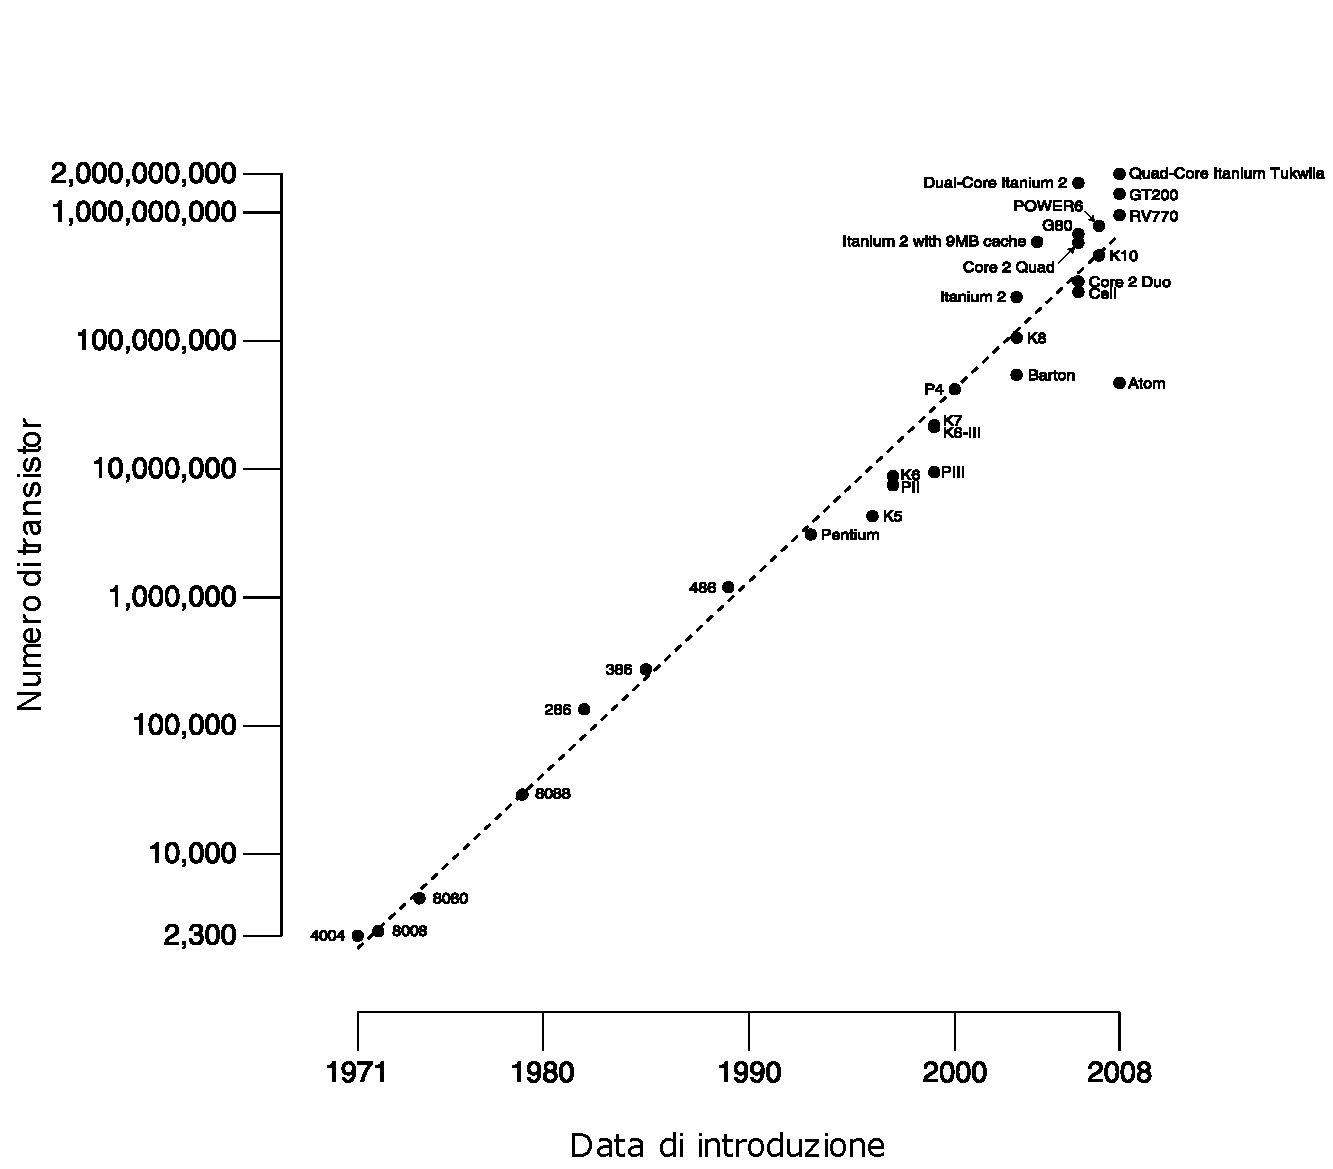
\includegraphics[width=\textwidth]{img/moore-law}
\caption{Numero di transistor per microprocessore dal 1971 al 2008 (fonte: Wikipedia).\label{fig:moore-law}}
\end{center}
\end{figure}

D'altro canto, i produttori di \ac{GPU} hanno adottato anch'essi da tempo delle architetture basate su molteplici unità di calcolo parallele. Infatti le operazioni più pesanti che avvengono nell'ambito della grafica tridimensionale sono di tipo \ac{SIMD} e un elevato numero di core è fondamentale per la loro velocizzazione. Poiché attualmente le \ac{GPU} hanno un numero di core superiore a quello delle \ac{CPU} questo tipo di architettura viene definito many-core.

Nei computer odierni sono quasi sempre presenti unità di calcolo molteplici ed eterogenee, ciascuna formata da un numero variabile di core. Lato software diventa quindi fondamentale adottare paradigmi, tecniche e strumenti di programmazione parallela che riescano a sfruttare al meglio le risorse computazionali disponibili. In effetti, secondo la Legge di Amdahl, il limite superiore all'incremento di prestazioni di un software che sfrutta più risorse di calcolo contemporaneamente è proporzionale alla frazione dello stesso che può essere parallelizzata.

Nella pratica però la maggior parte dei programmi per scopi non scientifici non è stata scritta per fare uso di architetture parallele. Ciò avviene per diversi motivi, tra cui:
\begin{enumerate}
\item la programmazione parallela è molto più complessa di quella seriale;
\item gli strumenti per la programmazione parallela sono più complicati rispetto a quelli per la programmazione seriale.
\end{enumerate}

Per supportare la diffusione del proprio hardware per il calcolo parallelo i produttori stanno cercando di fornire un'infrastruttura software appropriata: ad esempio la NVIDIA Corporation fornisce un \ac{SDK} per la scrittura di programmi in grado di sfruttare le sue \ac{GPU} basate sulla \ac{CUDA} per calcoli non necessariamente legati alla grafica. Questa soluzione consente di sfruttare soltanto le \ac{GPU} della NVIDIA Corporation, tralasciando quelle della concorrenza e le \ac{CPU} in genere; il supporto di quest'ultime è delegato ai comuni strumenti di programmazione.

La tendenza a sfruttare le \ac{GPU} per calcoli non strettamente correlati ai loro compiti originari viene spesso indicata con l'espressione \ac{GPGPU}.

Anche l'Università degli Studi di Perugia si sta muovendo nell'ambito \ac{GPGPU}. 
Si è recentemente costituito un gruppo di lavoro che unisce ricercatori di varie discipline che hanno deciso di effettuare un'azione sinergica al fine di creare un contesto locale che offra la possibilità di realizzare progetti importanti su architetture hardware innovative. Il gruppo di lavoro coinvolge i Dipartimenti di Fisica, Chimica e Matematica e Informatica ed è coinvolto su diversi fronti e progetti. In particolare presso il Dipartimento di Fisica e l'\ac{INFN} si sta portando avanti il progetto \ac{MaCGO}, il quale si propone di sfruttare in modo ottimale i sistemi multi/many-core per calcoli nell'ambito dell'astronomia delle onde gravitazionali\footnote{Questa branca emergente dell'astronomia studia corpi celesti come buchi neri o stelle di neutroni grazie alla misurazione delle onde gravitazionali.}.

\chapter{OpenCL}
\linespread{1}
\epigraph{\textit{The limits of your language are the limits of your world.}}{L. Wittgenstein}
\linespread{1.3}

\begin{figure}[h]
\begin{center}
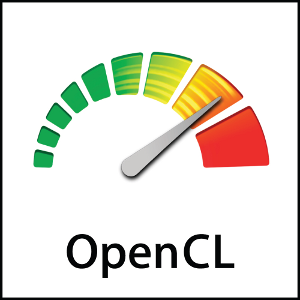
\includegraphics[width=150px]{img/opencl-logo}
\caption{Il logo di OpenCL.\label{fig:opencl-logo}}
\end{center}
\end{figure}

\ac{OpenCL} è uno standard creato dal Kronos Group che definisce un ambiente di programmazione parallela multipiattaforma in grado di sfruttare con un'interfaccia uniforme \ac{CPU}, \ac{GPU} e altri dispositivi di calcolo\cite{bib:opencl}. Il Kronos Group comprende organizzazioni come AMD, NVIDIA, Intel, Apple e Los Alamos National Laboratory.

\ac{OpenCL} definisce un'\ac{API} per gestire le computazioni sui diversi dispositivi di calcolo e un linguaggio per la scrittura dei programmi che dovranno essere eseguiti sugli stessi.

Per poter comprendere e usare efficacemente \ac{OpenCL} è necessario guardarlo da diversi punti di vista:
\begin{enumerate}
\item modello della piattaforma;
\item modello di esecuzione;
\item modello della memoria;
\item modello di programmazione.
\end{enumerate}

\section{Modello della piattaforma}
\label{sec:opencl-platform}

\begin{figure}[h]
\begin{center}
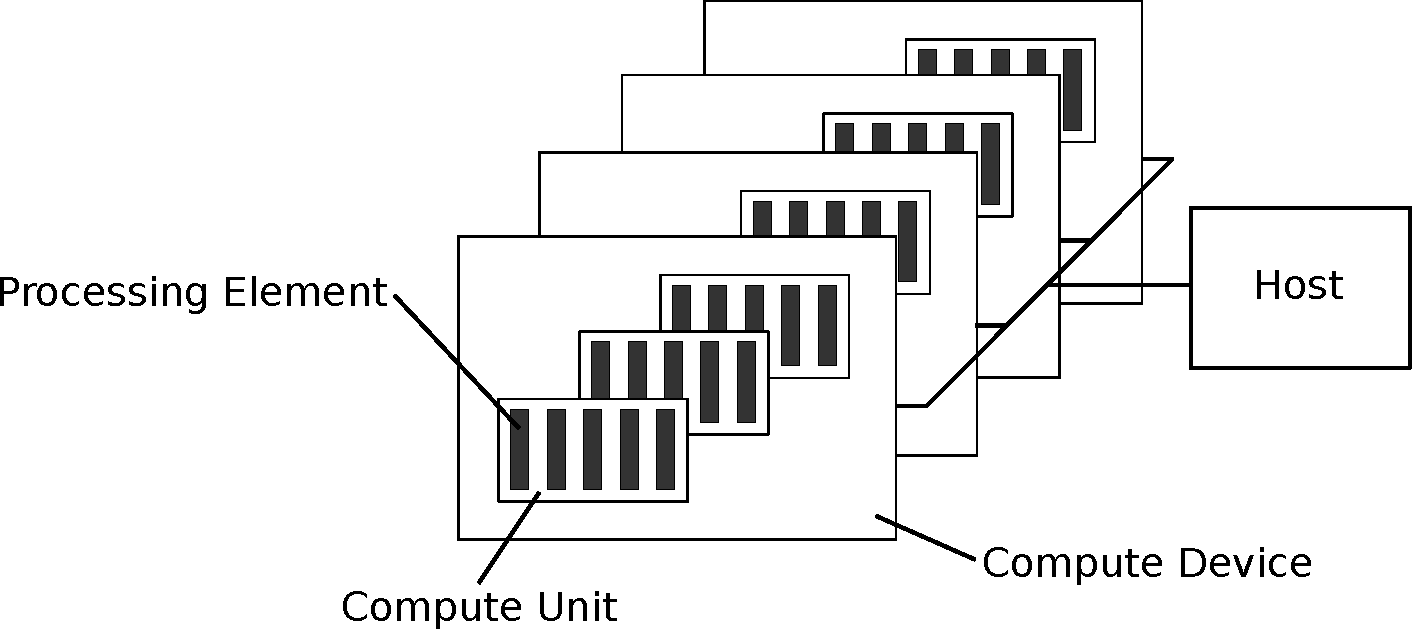
\includegraphics[width=\textwidth]{img/opencl-platform-model}
\caption{Il modello della piattaforma di \ac{OpenCL}.\label{fig:opencl-platform-model}}
\end{center}
\end{figure}

La figura \ref{fig:opencl-platform-model} rappresenta il modello della piattaforma di \ac{OpenCL}. In particolare, in tale modello viene definito un host (normalmente un comune computer) connesso a uno o più device (di solito \ac{CPU} o \ac{GPU}). Un device contiene a sua volta una o più \ac{CU}; una \ac{CU} è ulteriormente divisa in \ac{PE}, ovvero i dispositivi che eseguono effettivamente i calcoli.

Il flusso d'esecuzione di un'applicazione \ac{OpenCL} inizia nell'host; da qui l'applicazione invierà dei comandi affinché vengano eseguiti dei calcoli nei \ac{PE} di un particolare device. I \ac{PE} contenuti all'interno della medesima \ac{CU} possono eseguire un singolo flusso di istruzioni secondo uno di questi modelli:
\begin{description}
\item[Single Instruction, Multiple Data:] i \ac{PE} eseguono lo stesso programma su dati diversi condividendo un medesimo program counter;
\item[Single Program, Multiple Data:] i \ac{PE} eseguono lo stesso programma su dati diversi, ciascuno il proprio program counter indipendente da quello degli altri.
\end{description}

\section{Modello di esecuzione}
\label{sec:opencl-execution-model}

Il flusso di esecuzione di un programma basato su \ac{OpenCL} è suddiviso in due parti:
\begin{enumerate}
\item un programma eseguito nell'host;
\item una o più funzioni eseguite dei device, dette kernel.
\end{enumerate}

Il programma eseguito nell'host prepara l'esecuzione dei vari kernel, definendo i device da utilizzare, il tipo di parallelismo, i dati in input e quelli in output.

Il nodo principale del modello di esecuzione \ac{OpenCL} è definito da come vengono eseguiti i kernel. Quando il programma nell'host richiede l'esecuzione di un kernel viene definito uno spazio degli indici e viene eseguita un'istanza del kernel per ogni punto di tale spazio. Ciascuna istanza viene definita con il nome di work-item ed è identificata proprio dal punto nello spazio degli indici cui è associata: questo identificatore è anche detto global ID. Ciascun work-item esegue il codice dello stesso kernel ma il flusso d'esecuzione può non essere sincronizzato a causa di costrutti condizionali o cicli con condizioni variabili.

I work-item sono raggruppati in work-group; questi rappresentano una decomposizione a grana più grossa dello spazio degli indici. Ciascun work-group è identificato univocamente con un work-group ID e i suoi work-item hanno ciascuno un local ID, ovvero un identificatore univoco soltanto all'interno del work-group stesso.

Da quanto detto negli ultimi due paragrafi si evince che un work-item può essere identificato univocamente in due modi:
\begin{enumerate}
\item dal proprio global ID;
\item da una combinazione del suo local ID e dell'identificatore del work-group cui esso appartiene.
\end{enumerate}

Con riferimento al modello della piattaforma, ciascun work-item di un dato work-group viene eseguito in modo concorrente in un \ac{PE} di una singola \ac{CU}.

Lo spazio degli indici può essere multidimensionale. La versione 1.0 della specifica \ac{OpenCL} consente di avere spazi di una, due o tre dimensioni\cite{bib:opencl}; questo limite è riconducibile al compito principale delle \ac{GPU}, l'elaborazione di grafica tridimensionale. Lo spazio degli indici di \ac{OpenCL} viene chiamato \ac{NDRange} ed è implementato come vettore di lunghezza N in cui ciascuna componente specifica l'estensione della dimensione corrispondente. Ne consegue che anche i global ID, i local ID e i work-group ID sono dei vettori di N elementi. Seguendo la convenzione tipica del linguaggio C, ciascuna componente di un global ID può assumere un valore che va da 0 all'estensione della dimensione corrispondente meno uno. Lo stesso vale per local ID e work-group ID, considerando le opportune limitazioni superiori. 

Un esempio bidimensionale sulla relazione tra global ID, work-group ID e local ID è visibile in figura \ref{fig:opencl-ndrange}. Sono noti lo spazio degli indici globale $(G_x, G_y)$ e la dimensione di ciascun work-group $(S_x, S_y)$, dai quali si possono ricavare diverse informazioni. Ad esempio, il numero totale di work-item è dato dal prodotto $G_xG_y$ e il numero di work-group è pari a $\frac{G_x}{S_x}\frac{G_y}{S_y}$. Introducendo anche il local ID di un work-item, $(s_x, s_y)$, nonché il suo work-group ID $(w_x, w_y)$, si può anche mostrare la relazione che lega global ID, work-group ID e local ID:

\begin{center}
\begin{math}
(g_x, g_y) = (w_xS_x + s_x, w_yS_y + s_y)
\end{math}
\end{center}

\begin{figure}[t]
\begin{center}
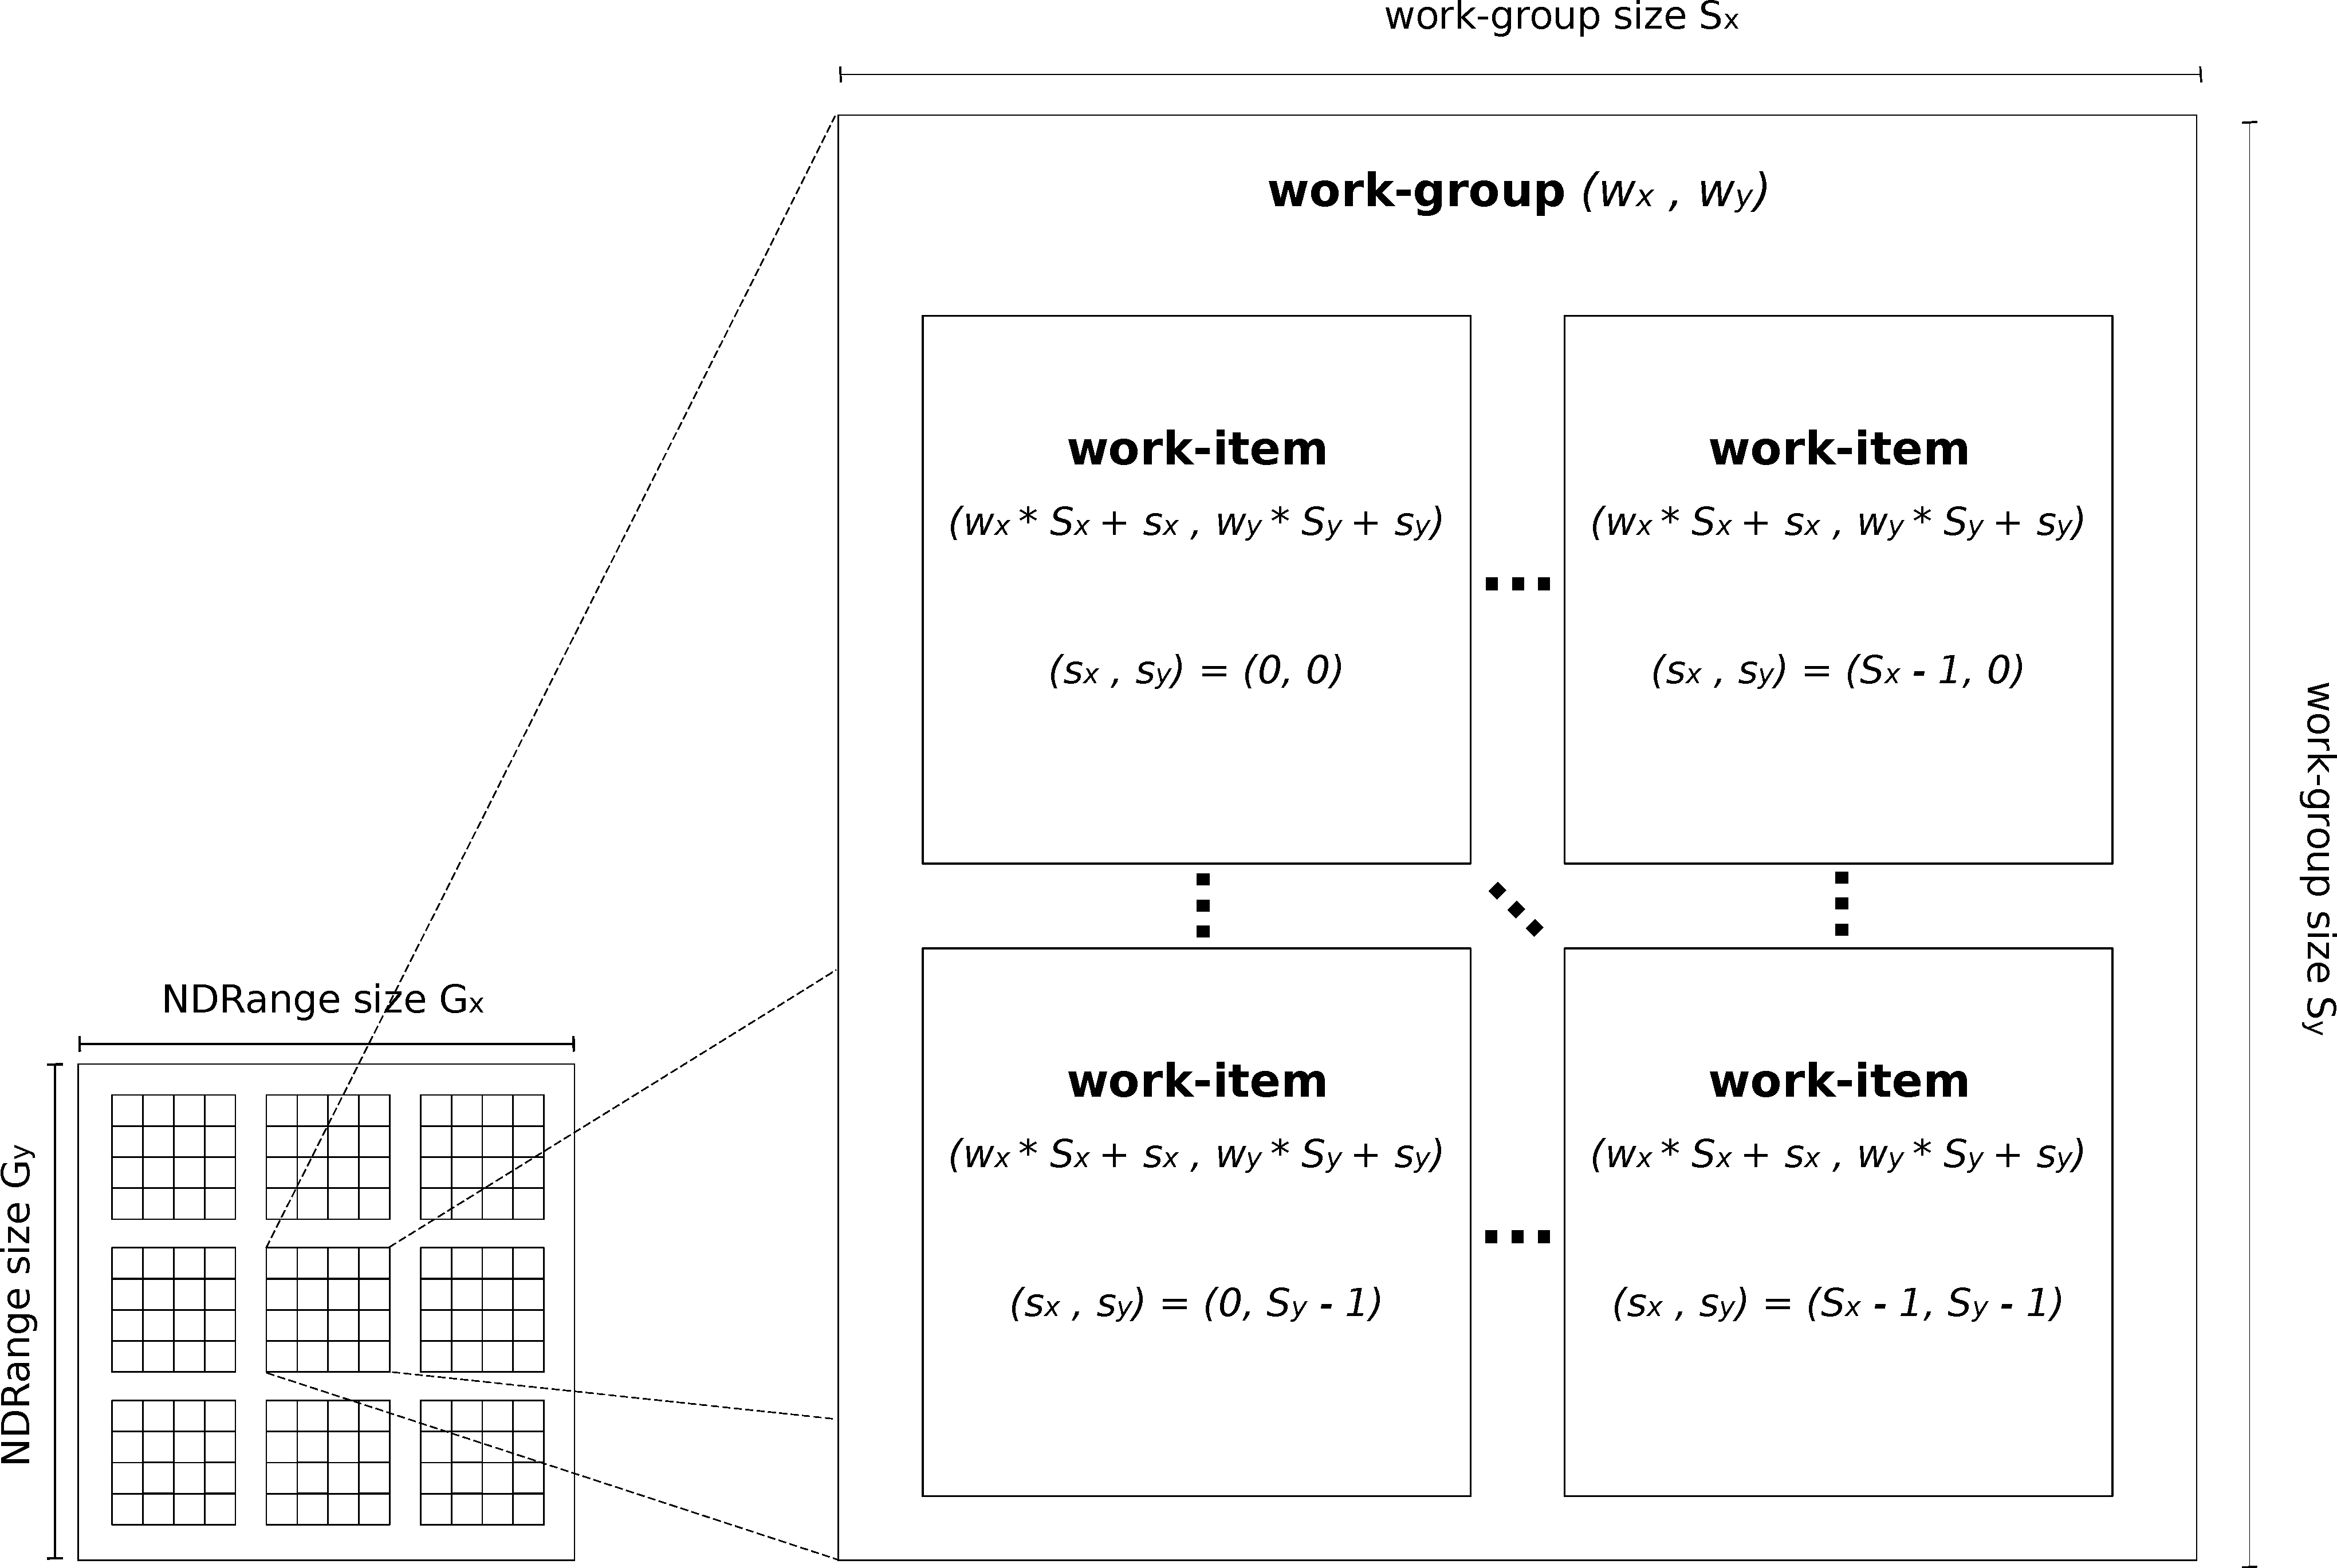
\includegraphics[width=\textwidth]{img/opencl-ndrange}
\caption{Un esempio di spazio degli indici bidimensionale; si noti la relazione tra global ID, work-group ID e local ID.\label{fig:opencl-ndrange}}
\end{center}
\end{figure}

\subsection{Code di comandi e contesti}
\label{sec:opencl-code-contesti}

Un kernel \ac{OpenCL} viene eseguito in un determinato contesto; sotto questa definizione sono raggruppate le seguenti risorse:
\begin{description}
\item[Device:] come già detto, si tratta dei dispositivi fisici su cui andranno in esecuzione i kernel \ac{OpenCL};
\item[Kernel:] le funzioni \ac{OpenCL} eseguite nei device;
\item[Program Object:] il codice sorgente e quello macchina dei programmi che implementano i kernel;
\item[Memory Object:] servono a condividere dati tra il programma host e i kernel in esecuzione sui device.
\end{description}

Grazie all'\ac{API} \ac{OpenCL} il programma in esecuzione nell'host deve prima definire un contesto, quindi creare una coda di comandi che può contenere le seguenti tipologie di istruzioni:
\begin{enumerate}
\item esecuzione di un kernel;
\item lettura e scrittura della memoria dei device;
\item sincronizzazione tra comandi in coda.
\end{enumerate}

I comandi presenti nella coda vengono poi schedulati per l'esecuzione nel device prescelto. A causa di ciò l'esecuzione dei comandi da parte dell'host nei dispositivi \ac{OpenCL} è generalmente asincrona, tuttavia esistono delle apposite funzioni per la sincronizzazione host/device. Ciascun device esegue i comandi inviatigli mediante le code nell'ordine in cui li riceve; esistono tuttavia due modalità di esecuzione:
\begin{enumerate}
\item in ordine, ovvero ciascun comando viene eseguito completamente prima che inizi il successivo;
\item fuori ordine, ovvero lo scheduler del device non attende il completamento di un comando per lanciare il successivo.
\end{enumerate}

I comandi riguardanti l'esecuzione di un kernel oppure le operazioni sulla memoria possono essere associati a degli eventi\label{pag:opencl-event}; questi possono essere usati per coordinare l'esecuzione dei vari comandi o per rilevare il tempo impiegato per il loro completamento.

\section{Modello della memoria}
\label{sec:opencl-memory}

\ac{OpenCL} definisce quattro tipi di memoria:
\begin{description}
\item[Global Memory:] è leggibile e scrivibile da tutti i work-item di qualsiasi work-group nonché dal programma in esecuzione nell'host; potrebbe essere dotata di cache.
\item[Constant Memory:] è solo leggibile dai work-item mentre il programma in esecuzione nell'host può anche scrivervi; potrebbe essere dotata di cache\footnote{Secondo quanto riportato in \cite{bib:nvidia} tutte le schede video della NVIDIA Corporation hanno una Constant Memory dotata di cache.}.
\item[Local Memory:] è locale a un singolo work-group, quindi può essere usata per variabili che sono condivise da tutti i work-item dello stesso work-group. Nel caso di device di tipo \ac{GPU} è solitamente una memoria dedicata, mentre per le \ac{CPU} viene fatta corrispondere a una regione della Global Memory.
\item[Private Memory:] ciascun work-item ha una propria porzione di memoria privata, distinta da quella degli altri, nella quale può leggere e scrivere a piacimento.
\end{description}

Nella tabella \ref{tab:opencl-memory-access} sono riassunte le modalità di accesso alle varie tipologie di memoria da parte di host e device, mentre in figura \ref{fig:opencl-memory-model} è rappresentata graficamente la relazione tra il modello della memoria e quello della piattaforma.

\begin{table}[p]
\begin{center}
\begin{tabular}{|l|l|l|l|l|}
\hline
 & \textbf{Global} &  \textbf{Constant} & \textbf{Local} & \textbf{Private} \\
\hline
\textbf{Host} & lettura   & lettura   & non accessibile & non accessibile \\
              & scrittura & scrittura &                 &                 \\
\hline
\textbf{Device} & lettura   & lettura & lettura   & lettura   \\
                & scrittura &         & scrittura & scrittura \\
\hline
\end{tabular}
\caption{Modalità di accesso alla memoria \ac{OpenCL} da parte di host e device.\label{tab:opencl-memory-access}}
\end{center}
\end{table}

\begin{figure}[p]
\begin{center}
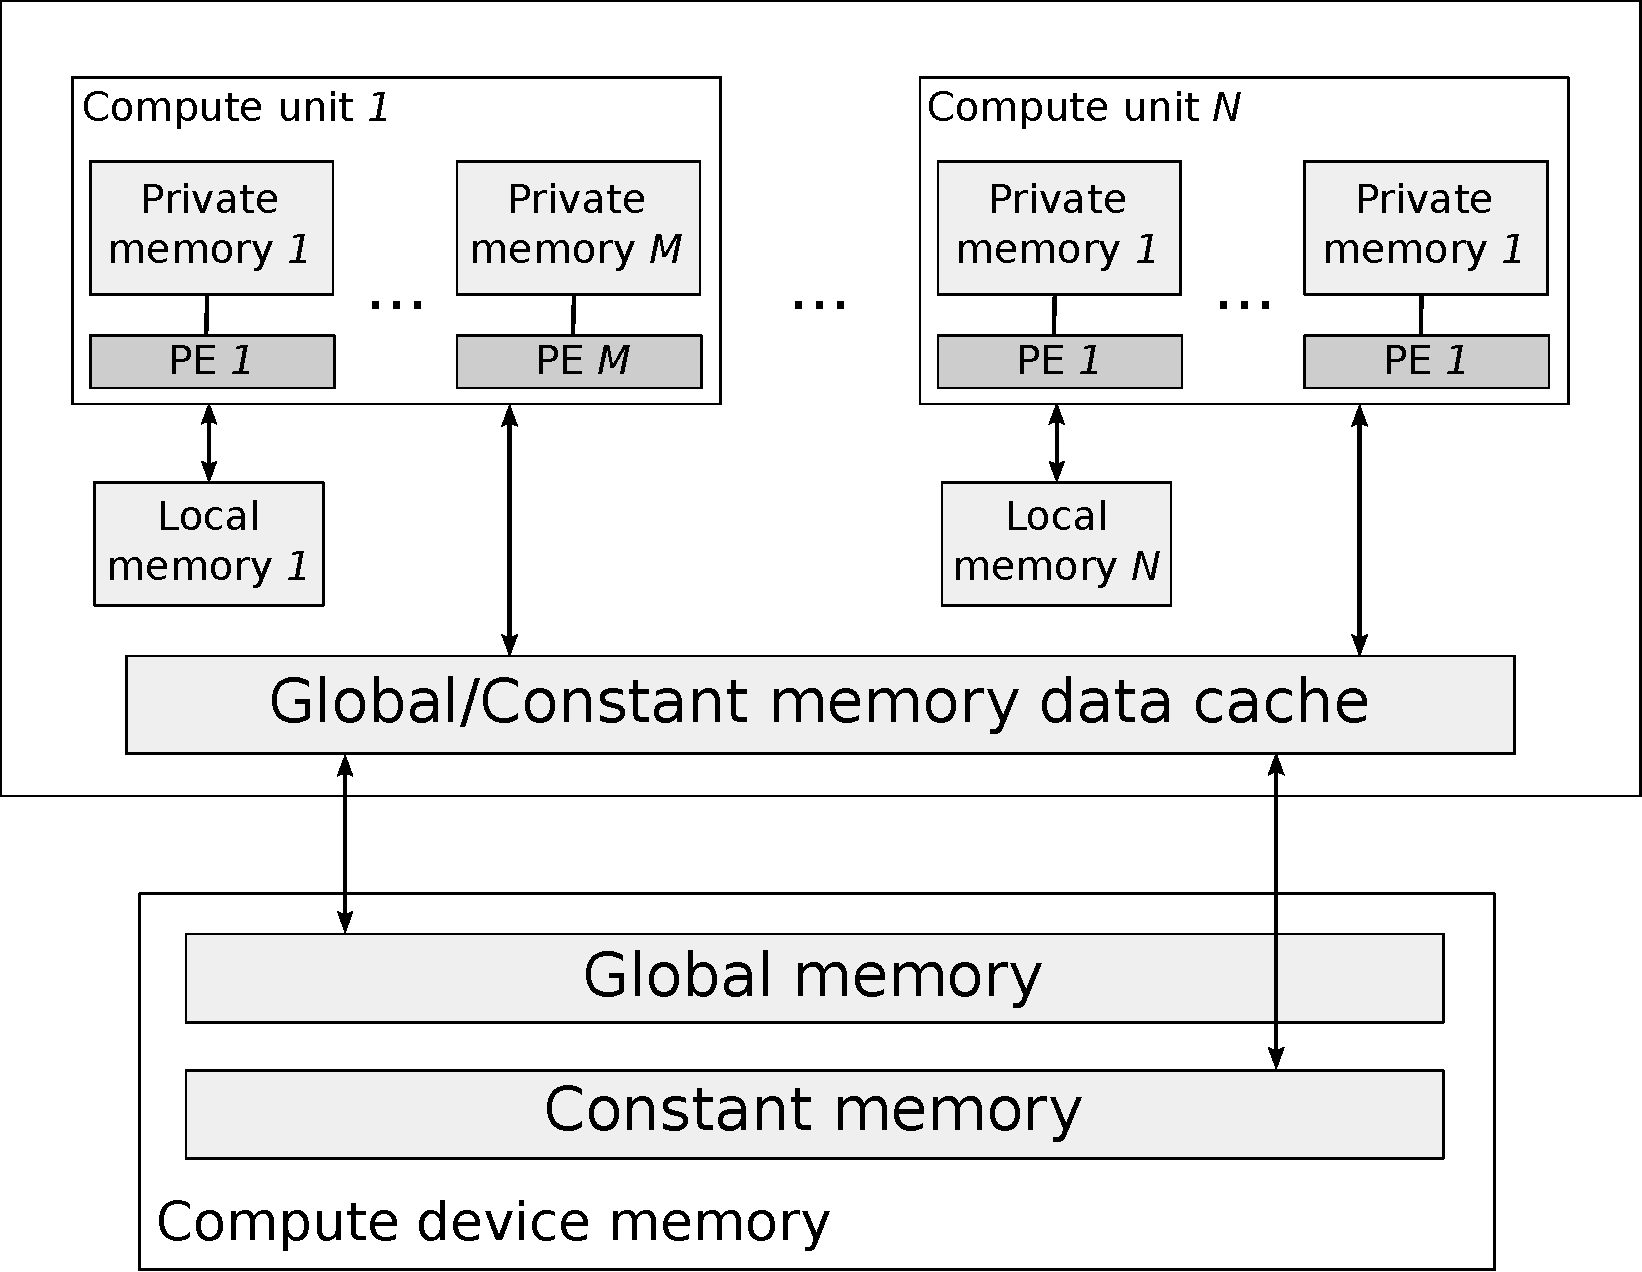
\includegraphics[width=\textwidth]{img/opencl-memory-model}
\caption{Relazione tra i modelli \ac{OpenCL} della piattaforma e della memoria.\label{fig:opencl-memory-model}}
\end{center}
\end{figure}

Il programma in esecuzione nell'host usa la consueta \ac{API} \ac{OpenCL} per creare dei Memory Object che fungeranno da interfaccia verso la Global Memory e per mettere in una coda dei comandi per effettuare operazioni di lettura e scrittura su tali oggetti.

Lettura e scrittura dalla memoria dell'host a quella del device possono avvenire in due modi: copiando esplicitamente i dati o creando delle corrispondenze tra regioni di memoria dell'host e del device (in inglese questa operazione viene definita mapping).

Per copiare i dati esplicitamente il programma in esecuzione sull'host mette in coda dei comandi per il trasferimento dei dati; come già detto, questi comandi possono essere eseguiti sia in modo bloccante che in modo non bloccante.

Per finire, una nota molto importante sul modello di memoria \ac{OpenCL}, riportata direttamente dalla specifica \ac{OpenCL} \cite{bib:opencl}:

\begin{quote}
\textit{``OpenCL uses a relaxed consistency memory model; i.e. the state of memory visible to a work-item is not guaranteed to be consistent across the collection of work-items at all times''}
\end{quote}

Le uniche garanzie che si hanno a proposito della memoria sui device sono:
\begin{enumerate}
\item la Private Memory è coerente rispetto alle operazioni di lettura e scrittura all'interno di un singolo work-item;
\item la Local Memory è coerente per tutti i work-item dello stesso work-group;
\item la Global Memory è coerente per tutti i work-item dello stesso work-group ma non ci sono garanzie circa la coerenza tra work-item di work-group diversi che stanno eseguendo il medesimo kernel.
\end{enumerate}

Qualora il programmatore necessiti di un tipo di coerenza non fornito direttamente da \ac{OpenCL} dovrà usare le funzioni di sincronizzazione per ottenere il risultato desiderato.

\section{Modello di programmazione}

\ac{OpenCL} supporta tre modelli per la programmazione parallela:
\begin{enumerate}
\item parallelismo rispetto ai dati;
\item parallelismo rispetto ai task;
\item un ibrido dei due modelli precedenti.
\end{enumerate}

Tra questi il modello maggiormente supportato è sicuramente il parallelismo rispetto ai dati.

\subsection{Parallelismo rispetto ai dati}
\label{sec:opencl-data-parallel}

In questo caso la computazione viene definita in termini di istruzioni applicate a più elementi di un Memory Object. Lo spazio degli indici, definito nella sezione \ref{sec:opencl-execution-model}, viene usato per stabilire il numero di work-item e la loro corrispondenza alle diverse parti dei dati in memoria; ciascun work-item potrà poi operare parallelamente rispetto agli altri sulla sua sezione dei dati, a seconda delle unità di calcolo effettivamente disponibili nel device.

\ac{OpenCL} fornisce al programmatore due modi di suddividere i dati tra i vari work-item:
\begin{enumerate}
\item specificando sia il numero totale di work-item che la loro suddivisione in work-group;
\item specificando soltanto il numero totale di work-item, lasciando che sia l'implementazione di \ac{OpenCL} a gestire la loro ripartizione in work-group.
\end{enumerate}

Come già detto nella sezione \ref{sec:opencl-platform} il parallelismo rispetto ai dati può essere sia di tipo \ac{SIMD} che di tipo \ac{SPMD}.

\subsection{Parallelismo rispetto ai task}

In questo caso vengono eseguite diverse istanze di un kernel indipendentemente da qualsiasi spazio degli indici. Questo tipo di astrazione potrebbe essere paragonato all'esecuzione di un kernel con un singolo work-group contenente a sua volta un unico work-item.

Per ottenere questo tipo di parallelismo vengono generalmente sfruttate le code dei comandi, inserendo in esse più istanze di kernel.

\subsection{Sincronizzazione}

\ac{OpenCL} definisce due tipologie di sincronizzazione:
\begin{enumerate}
\item tra work-item del medesimo work-group;
\item tra comandi messi in coda in una o più code associate a un singolo contesto.
\end{enumerate}

Non esiste invece alcun meccanismo di sincronizzazione tra work-group.

La sincronizzazione tra work-item dello stesso work-group viene ottenuta mediante una barriera a livello di work-group: ciascun work-item deve eseguire la barriera e attendere che tutti gli altri lo abbiano fatto a loro volta.

La sincronizzazione tra i comandi delle code può essere ottenuta in due modi:
\begin{enumerate}
\item mediante barriere a livello di coda, che però garantiscono il sincronismo soltanto per i comandi contenuti all'interno della medesima coda;
\item mediante l'attesa rispetto a un evento (vedi la sottosezione \ref{pag:opencl-event}); questo metodo funziona anche tra code diverse.
\end{enumerate}

\section{Estensioni del linguaggio C per i kernel OpenCL}
\label{sec:opencl-c99}

Per la creazione dei kernel, \ac{OpenCL} definisce un linguaggio basato sullo standard ISO/IEC 9899:1999, conosciuto informalmente come C99, con diverse estensioni per la programmazione parallela. Le seguenti sono particolarmente degne di attenzione: 
\begin{enumerate}
\item tipi di dato vettoriali di lunghezza 2, 4, 8 o 16 che consentono di effettuare operazioni sui singoli elementi in parallelo qualora il device lo supporti;
\item tipi di dato per la rappresentazione di immagini a due o tre dimensioni;
\item controllo accurato delle operazioni di conversione tra tipi di dato;
\item conformità dei tipi di dato in virgola mobile allo standard IEEE-754;
\item modificatori aggiuntivi per variabili e argomenti di funzione al fine di specificare l'area di memoria in cui sono allocati (\verb|__global|, \verb|__constant|, \verb|__local| e \verb|__private|).
\end{enumerate}

La definizione delle funzioni che implementano i kernel, la cui esecuzione sul device è evocabile dal programma sull'host, deve essere preceduta dal modificatore \verb|__kernel|.

D'altro canto il C di OpenCL presenta anche diverse limitazioni, anche rispetto al C99, tra cui:
\begin{enumerate}
\item gli argomenti di tipo puntatore che compaiono in una funzione kernel devono essere preceduti dal qualificatore \verb|__global|, \verb|__constant| o \verb|__local|;
\item gli argomenti di tipo puntatore di una funzione kernel non possono avere più di un livello di indirezione (nessun puntatore a puntatore, quindi);
\item un puntatore definito come \verb|__global|, \verb|__constant| o \verb|__local| può essere assegnato soltanto a un altro puntatore definito con il medesimo qualificatore;
\item non è possibile usare puntatori a funzioni;
\item la maggior parte degli header della libreria standard C99 non può essere usata;
\item non sono supportati i qualificatori \verb|extern|, \verb|static| e \verb|auto|;
\item non è possibile usare la ricorsione;
\item le funzioni kernel devono sempre essere di tipo \verb|void|;
\item non è possibile scrivere in aree di memoria rappresentate da un puntatore di un tipo di dato la cui dimensione è inferiore a 32 bit\footnote{In realtà è possibile fare ciò tramite delle estensioni, ma le implementazioni \ac{OpenCL} non sono tenute a supportarle.}.
\end{enumerate}

\section{Implementazioni}
\label{sec:opencl-impl}

Lo standard \ac{OpenCL} è stato implementato da diversi produttori, tra cui:
\begin{description}
\item[NVIDIA,] per le proprie \ac{GPU}\footnote{\url{http://www.nvidia.com/object/cuda_opencl.html}};
\item[AMD,] sia per le proprie \ac{GPU} che per le principali \ac{CPU}\footnote{\url{http://ati.amd.com/technology/streamcomputing/opencl.html}};
\item[IBM,] per i suoi processori con architettura POWER\footnote{\url{http://www.alphaworks.ibm.com/tech/opencl}}.
\end{description}

Ciascuna implementazione fornisce i seguenti componenti:
\begin{enumerate}
\item driver per l'uso dei dispositivi di calcolo da parte del programma in esecuzione nell'host;
\item implementazione dell'\ac{API} \ac{OpenCL};
\item compilatore per kernel \ac{OpenCL}.
\end{enumerate}

\chapter{Advanced Encryption Standard}
\label{cha:aes}
\linespread{1}
\epigraph{\textit{There are two types of encryption: one that will prevent your sister from reading your diary and one that will prevent your government. }}{B. Schneier}
\linespread{1.3}
L'\ac{AES} è l'attuale standard per la crittografia simmetrica del governo statunitense poiché è stato dichiarato \ac{FIPS} dal \ac{NIST} dopo un approfondito processo di selezione\cite{bib:fips-197}.

\ac{AES} è basato sull'algoritmo per la cifratura simmetrica Rijndael\footnote{Il nome Rijndael è una combinazione dei nomi fiamminghi dei suoi autori; si pronuncia ``rèin-daal''.} ideato dai crittografi belgi Joan Daemen and Vincent Rijmen; Rijndael è stato scelto tra le diverse proposte perché rappresenta un buon compromesso tra sicurezza e velocità di elaborazione, sia nelle sue implementazioni software che in quelle hardware.\cite{bib:aes-report}.

\begin{table}[h]
\begin{center}
\begin{tabular}{|l|l|l|l|l|}
\hline
\textbf{Lunghezza chiave} &  \textbf{Numero round} \\
\hline
128 bit & 10 \\
\hline
192 bit & 12 \\
\hline
256 bit & 14 \\
\hline
\end{tabular}
\caption{Numero di round in relazione alla lunghezza della chiave \ac{AES}.\label{tab:aes-rounds}}
\end{center}
\end{table}

\ac{AES} lavora su blocchi di dati di 128 bit e consente di usare chiavi di tre lunghezze: 128, 192 o 256 bit. La sua struttura è quella di un algoritmo crittografico iterativo; il numero di round dipende dalla lunghezza della chiave (vedi tabella \ref{tab:aes-rounds}).

Da un punto di vista molto astratto, l'algoritmo di cifratura \ac{AES} può essere descritto dal codice \ref{cod:aes-encrypt}.

\vspace*{10pt}
\begin{figure}
\begin{lstlisting}[caption=\textit{Procedura di cifratura AES.},label={cod:aes-encrypt},language=Pascal]
State = input

AddRoundKey(State, RoundKey[0])

for r = 1 to rounds-1
	SubBytes(State)
	ShiftRows(State)
	MixColumns(State)
	AddRoundKey(State, RoundKey[r])
end

SubBytes(State)
ShiftRows(State)
AddRoundKey(State, RoundKey[rounds])

output = State
\end{lstlisting}
\end{figure}

La variabile \textit{input} rappresenta il blocco di dati in chiaro di 128 bit mentre \textit{output} è il corrispondente blocco cifrato. Le quattro procedure di base, \textit{AddRoundKey}, \textit{SubBytes}, \textit{ShiftRows} e \textit{MixColumns} sono tutte operazioni che modificano la variabile \textit{State}.

Per ragioni che saranno chiare tra poco, conviene pensare alla variabile \textit{State}, di 128 bit ovvero 16 byte, come a una matrice quadrata di lato 4 byte.

L'algoritmo di decifratura, descritto nel codice di Figura \ref{cod:aes-decrypt}, utilizza le medesime funzioni o le loro inverse; ovviamente in questo caso \textit{input} è il blocco di dati cifrato e \textit{output} il corrispondente blocco in chiaro.

\vspace*{10pt}
\begin{figure}
\begin{lstlisting}[caption={\textit{Procedura di decifratura AES.}},label={cod:aes-decrypt},language=Pascal]
State = input

AddRoundKey(State, RoundKey[rounds])

for r = rounds-1 to 1
	InvShiftRows(State)
	InvSubBytes(State)
	AddRoundKey(State, RoundKey[r])
	MixColumns(State)
end

InvShiftRows(State)
InvSubBytes(State)
AddRoundKey(State, RoundKey[0])

output = State
\end{lstlisting}
\end{figure}

\section{ShiftRows}

\begin{figure}[h]
\begin{center}
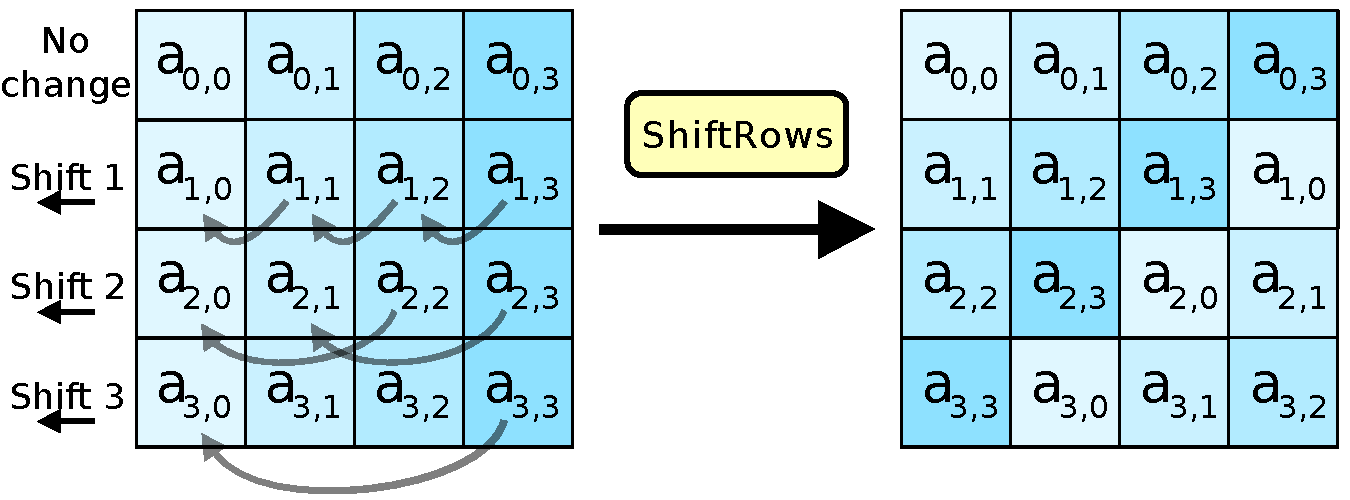
\includegraphics[width=0.7\textwidth]{img/shiftrows}
\caption{L'operazione ShiftRows di AES.\label{fig:aes-shiftrows}}
\end{center}
\end{figure}

La funzione \textit{ShiftRows} (figura \ref{fig:aes-shiftrows}) trasforma la matrice \textit{State} in questo modo:
\begin{enumerate}
\item la prima riga rimane invariata;
\item la seconda riga viene ruotata a sinistra di una posizione;
\item la terza riga viene ruotata a sinistra di due posizioni;
\item la quarta riga viene ruotata a sinistra di tre posizioni;
\end{enumerate}

La funzione inversa opera sulle stesse righe le medesime rotazioni ma in senso opposto, verso destra.

\section{SubBytes}
\label{sec:aes-subbytes}

\begin{figure}[h]
\begin{center}
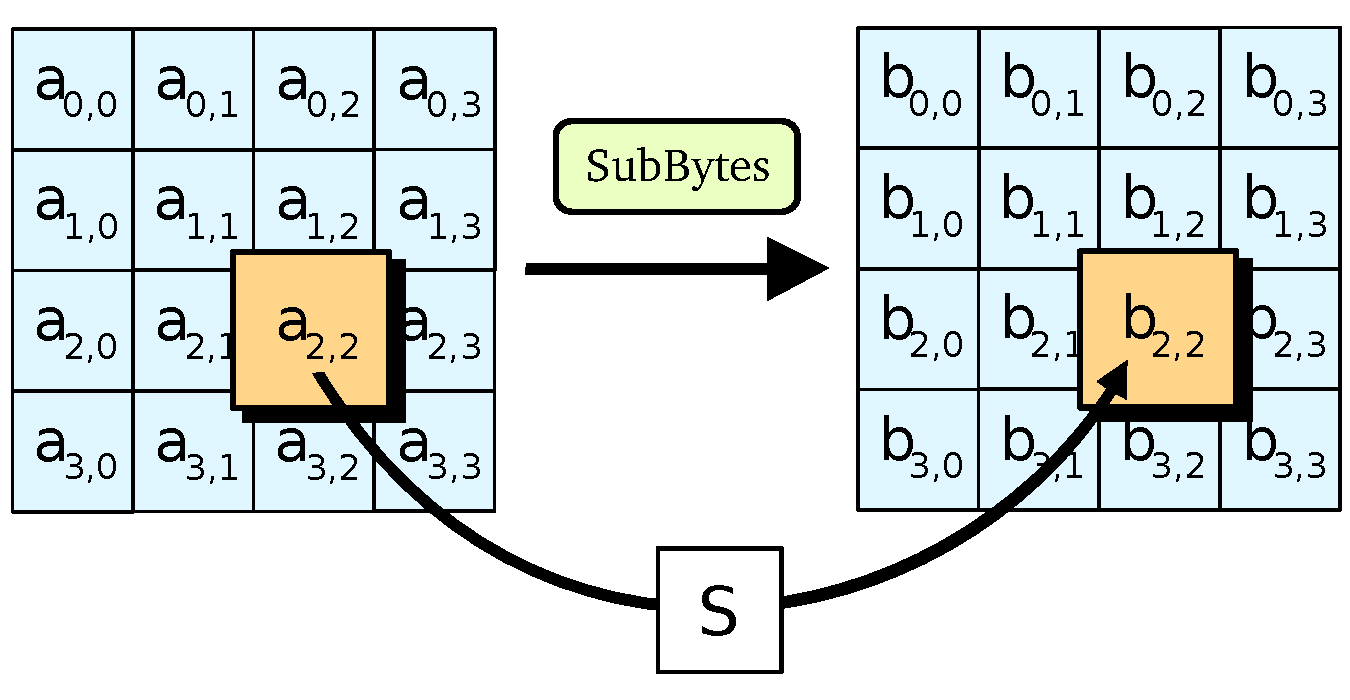
\includegraphics[width=0.7\textwidth]{img/subbytes}
\caption{L'operazione SubBytes di AES.\label{fig:aes-subbytes}}
\end{center}
\end{figure}

Dal punto di vista implementativo l'operazione di \textit{SubBytes} (figura \ref{fig:aes-subbytes}) non è altro che una classica \ac{S-box}, ovvero una sostituzione di tutti i byte della matrice \textit{State} con i corrispondenti valori di una tabella di 256 elementi; in realtà tale sostituzione può essere definita algebricamente. La formulazione algebrica della \ac{S-box} di \ac{AES} sfrutta il campo finito (o campo di Galois) basato sul seguente polinomio con valori in $Z_2$:
\begin{displaymath}
x^8 + x^4 + x^3 + x + 1
\end{displaymath}

La \ac{S-box} di \ac{AES} può essere sostituita concettualmente dall'operazione di inverso moltiplicativo nel campo finito di cui sopra, abbinata con una trasformazione affine. Questa particolare \ac{S-box} garantisce la non linearità ed è priva di punti fissi, rendendola immune da una classe di attacchi basata proprio su queste caratteristiche\cite{bib:stinson}.

La \ac{S-box} inversa è banalmente definita a partire da quella appena descritta.

\section{MixColumns}

\begin{figure}[h]
\begin{center}
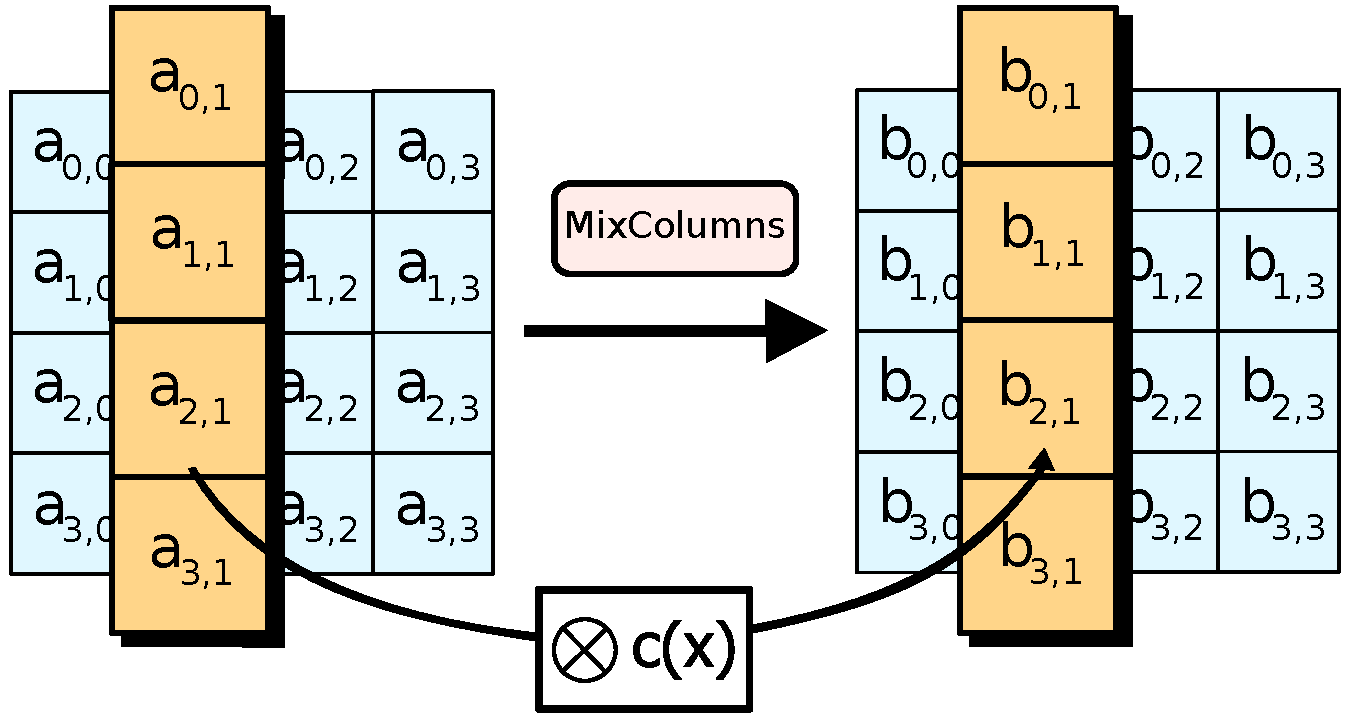
\includegraphics[width=0.7\textwidth]{img/mixcolumns}
\caption{L'operazione MixColumns di AES.\label{fig:aes-mixcolumns}}
\end{center}
\end{figure}

La funzione \textit{MixColumns} (figura \ref{fig:aes-mixcolumns}) opera sulle quattro colonne della matrice \textit{State}. Ogni colonna viene rimpiazzata dal risultato della sua moltiplicazione per una particolare matrice; le operazioni si svolgono nel campo finito descritto nella sezione \ref{sec:aes-subbytes}.

\section{AddRoundKey}

\begin{figure}[h]
\begin{center}
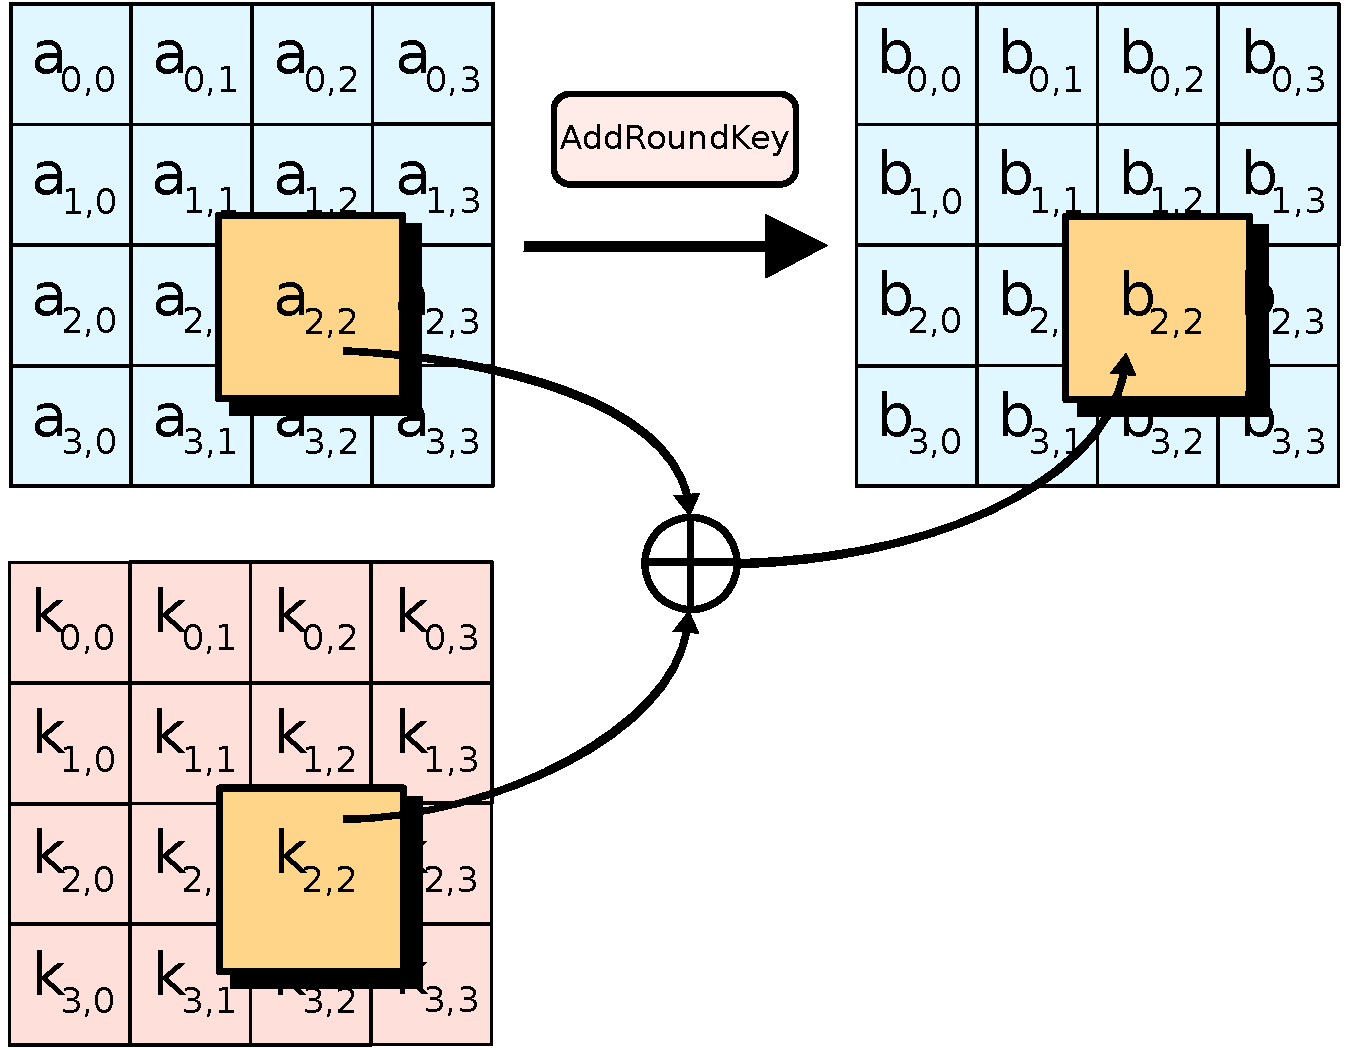
\includegraphics[width=0.7\textwidth]{img/addroundkey}
\caption{L'operazione AddRoundKey di AES.\label{fig:aes-addroundkey}}
\end{center}
\end{figure}

La funzione \textit{AddRoundKey} (figura \ref{fig:aes-addroundkey}) consiste in un semplice XOR della matrice \textit{State} con la sottochiave del round corrente. La generazione delle sottochiavi, tante quante il numero di round più uno, è compito della procedura di espansione della chiave descritta nella sezione \ref{sec:aes-key-schedule}. In questo caso la funzione coincide con la sua inversa, quello che cambia all'atto della decifratura è l'ordine con cui vengono applicate le varie sottochiavi.

\section{Espansione della chiave}
\label{sec:aes-key-schedule}

Il processo di espansione della chiave coinvolge la \ac{S-box} descritta nella sezione \ref{sec:aes-subbytes} e due ulteriori funzioni:
\begin{description}
\item[Rotate:] ruota di 1 byte verso sinistra una parola di 4 byte.
\item[Rcon:] esegue l'elevamento a potenza di un byte; sia il byte che le operazioni vengono considerati nel campo finito descritto nella sezione \ref{sec:aes-subbytes}.
\end{description}

Bisogna inoltre definire tre valori:
\begin{description}
\item[Nk:] la dimensione in bit della chiave divisa per 32;
\item[Nb:] dimensione in byte della chiave;
\item[Nr:] il numero di round (vedi tabella \ref{tab:aes-rounds}).
\end{description}

L'algoritmo completo per l'espansione della chiave è riportato nel codice di Figura \ref{cod:aes-keyexpansion}.

\vspace*{10pt}
\begin{figure}
\begin{lstlisting}[caption={\textit{Procedura di espansione della chiave AES.}},label={cod:aes-keyexpansion},language=Pascal]
key = {la chiave, un array di byte}
w = {l'insieme delle sottochiavi, un array di byte}
temp = {array di 4 byte}
i = 0

while i < Nk
	w[i] = [key[4 * i], 
	        key[4 * i + 1], 
	        key[4 * i + 2], 
	        key[4 * i + 3]]
	i = i + 1
end

i = Nk

while i < Nb * (Nr + 1)
	temp = w[i - 1]
	
	if i mod Nk = 0
		temp = SubWord(RotWord(temp)) xor Rcon[i / Nk]
	else 
		if Nk > 6 and i mod Nk = 4
			temp = SubWord(temp)
		end
	
	w[i] = w[i - Nk] xor temp
	i = i + 1
end
\end{lstlisting}
\end{figure}

\section{Cenni sulla sicurezza dell'AES}

Già durante la gara indetta dal \ac{NIST}, \ac{AES} era stato violato rispettivamente fino a 7 round per chiavi a 128 bit, 8 per quelle a 192 bit e 9 per quelle a 256 bit\cite{bib:schneier}.

Nell 2009 ci sono stati due attacchi importanti di tipo ``related-key''; in questi casi lo svolgimento dell'attacco richiede l'osservazione del cifrario in azione con diverse chiavi sconosciute ma legate tra loro da una relazione matematica nota. Biryukov-Khovratovich-Nikolic hanno portato un attacco di complessità $2^{119}$ per chiavi di 256 bit e 192 bit\cite{bib:aes-attack1}; Biryukov, Dunkelman, Keller, Khovratovich, e Shamir hanno elaborato un attacco di complessità $2^{39}$ una versione a 9 round di \ac{AES} con chiave a 128 bit sfruttando soltanto due chiavi correlate\cite{bib:aes-attack2}.

\part{Fase sperimentale}

\chapter{Analisi e progettazione}
\linespread{1}
\epigraph{\textit{Simplicity is a great virtue but it requires hard work to achieve it and education to appreciate it.}}{E. W. Dijkstra}
\linespread{1.3}
\section{Struttura del parallelismo}
\label{sec:paes-parallelism}

Poiché \ac{AES} è un cifrario a blocchi, è estremamente naturale applicarvi un parallelismo sui dati che sfrutti proprio la suddivisione dei dati di input in blocchi.

PAES può istanziare un qualsiasi numero di work-item (\textit{global\_size}) e ricevere in ingresso un file formato da qualsiasi numero di blocchi. Confrontando queste due variabili possiamo avere tre situazioni, con conseguente ripartizione dei blocchi rispetto ai work-item:

\begin{description}
\item[\textit{global\_size} $=$ \textit{blocchi}:] ciascun work-item si occupa di applicare \ac{AES} a un blocco dell'input;
\item[\textit{global\_size} $>$ \textit{blocchi}:] \textit{blocchi} work-item si occupano di applicare \ac{AES} a un blocco dell'input, \textit{globalsize} $-$ \textit{blocchi} work-item non vengono schedulati;
\item[\textit{global\_size} $<$ \textit{blocchi}:] ciascun work-item applica \ac{AES} a $\frac{global\_size}{blocchi}$ blocchi; se il \textit{resto} della divisione è diverso da zero, \textit{resto} work-item dovranno occuparsi di un ulteriore blocco dell'input.
\end{description}

In poche parole PAES cerca di ripartire uniformemente i blocchi da cifrare tra i work-item disponibili senza porre vincoli artificiosi a queste due variabili. In questo modo è possibile dimensionare il numero di work-item a seconda delle peculiarità dell'hardware a disposizione.

In termini strettamente riguardanti \ac{OpenCL}, quanto scritto sopra equivale a definire uno spazio degli indici monodimensionale la cui grandezza non è necessariamente fissata a priori; anche la suddivisione dei work-item in work-group non è cablata nello schema di parallelismo ed è adattabile rispetto al dispositivo di calcolo usato di volta in volta. Il modello di suddivisione dei dati corrisponde al \ac{SPMD} (vedi sezione \ref{sec:opencl-data-parallel}) in quanto ciascun work-item è istanza del medesimo kernel ma il flusso di esecuzione può seguire percorsi differenti.

\section{Strumenti utilizzati}

La scelta di \ac{OpenCL} impone l'uso del suo dialetto C99 (vedi sezione \ref{sec:opencl-c99}) per la creazione dei kernel che saranno eseguiti nei device.

Per quanto concerne il programma lato host esistono \ac{API} \ac{OpenCL} per numerosi linguaggi di programmazione, ma quelle fornite dai produttori sono utilizzabili direttamente soltanto da programmi C o C++. Poiché lo stato delle diverse implementazioni di \ac{OpenCL} è in continua evoluzione, per evitare problemi dovuti alla sincronizzazione delle modifiche tra le \ac{API} originali e quelle dei vari binding, PAES sfrutta direttamente le \ac{API} C/C++ fornite dai produttori.

Il programma lato host è stato scritto con il linguaggio C99, ovvero la più recente evoluzione standardizzata dall'\ac{ISO} del C, le cui peculiarità utilizzate in PAES sono:
\begin{enumerate}
\item possibilità di commentare con la sequenza ``//'';
\item possibilità di dichiarare variabili in qualsiasi punto del programma;
\item introduzione di un tipo di dato booleano, ovvero un intero che può assumere soltanto i valori 0 e 1; qualora un altro intero venga convertito in booleano, se il suo valore è 0 rimane 0, se è diverso da 0 diventa 1. È così possibile mantenere la compatibilità con la rappresentazione dei valori booleani del C classico usando un tipo di dati più espressivo dei generici interi.
\end{enumerate}

Il compilatore di riferimento è il GCC, versione 4; sia i test che lo sviluppo sono stati eseguiti su sistemi Linux, sia a 32 bit che a 64 bit. Le implementazioni di \ac{OpenCL} utilizzate sono rispettivamente quella della NVIDIA Corporation e quella di AMD, nelle ultime versioni disponibili al momento della stesura di questo elaborato, rispettivamente la 2.3 e la 2.0.

Per quanto riguarda il programma in esecuzione nell'host sono stati ampiamente usati \ac{DDD}\footnote{\url{http://www.gnu.org/software/ddd/}} e Valgrind\footnote{\url{http://valgrind.org/}}: il primo è un'interfaccia grafica per molti debugger, tra quello usato durante lo sviluppo di PAES, il \ac{GDB}; Valgrind invece consente di eseguire un programma in un ambiente emulato per rilevare errori nell'allocazione e nell'uso della memoria, estremamente comuni nei programmi sviluppati in C.

Il codice è ampiamente documentato mediante l'uso di Doxygen\footnote{\url{http://www.stack.nl/~dimitri/doxygen/}}: si tratta di uno strumento che consente di inserire la documentazione dei vari metodi, costanti, tipi di dato, etc., direttamente all'interno del codice, esattamente come JavaDoc.

I programmi di test descritti nella sezione \ref{sec:test} sono basati su Python 2.6 e richiedono una shell compatibile con la Bourne Shell (es. la diffusissima BASH).

\section{Struttura dei file sorgenti}
\label{sec:paes-files}

PAES è formato da 7 file sorgenti, ciascuno con un ruolo ben preciso:
\begin{description}
\item[\textit{paes\_functions.c}:] contiene la funzione \textit{apply\_aes} che consente al programma lato host di eseguire la procedura \ac{AES} sul device \ac{OpenCL};
\item[\textit{paes\_functions.h}:] contiene i prototipi delle funzioni che sono esportate per l'uso esterno rispetto a \textit{paes\_functions.c}.
\item[\textit{paes.cl}:] contiene il kernel che esegue un round di \ac{AES} specificato dal programmatore sui dati passatigli in ingresso e le funzioni accessorie per assolvere questo compito;
\item[\textit{paes\_constants\_and\_datatypes.h}:] contiene le costanti e i tipi di dato non primitivi condivisi tra il programma lato host e il kernel \ac{OpenCL};
\item[\textit{paes\_size.h}:] contiene dei valori usati per determinare local e global size (vedi sottosezione \ref{subsec:paes-global-local-size});
\item[\textit{sha256.c}:] contiene un'implementazione della funzione di hashing SHA-256, utilizzata da PAES per trattare le password inserite dall'utente;
\item[\textit{sha256.h}:] contiene i prototipi delle funzioni esportate da \textit{sha256.c};
\item[\textit{paes.c}:] contiene la funzione \textit{main} e tutte le funzioni strettamente necessarie all'interfaccia a riga di comando del programma.
\end{description}

Insieme ai sorgenti, PAES comprende anche due file accessori:
\begin{description}
\item[\textit{doxygen.cfg}:] contiene la configurazione di Doxygen personalizzata per PAES;
\item[\textit{Makefile}:] contiene le regole per la compilazione di PAES e altri compiti secondari, come l'indentazione automatica del codice sorgente secondo lo standard K\&R.
\end{description}

\section{Interfaccia utente}
\label{sec:paes-cli}

Poiché PAES è un progetto con finalità principalmente di ricerca, la complessità dell'interfaccia utente è minima rispetto a quella del nucleo del programma. In effetti PAES è un semplice programma a riga di comando (vedi figura \ref{fig:paes-screenshot}) il cui comportamento è definito dalle opzioni specificate dall'utente descritte nella tabella \ref{tab:paes-opzioni}.

\begin{figure}[h]
\begin{center}
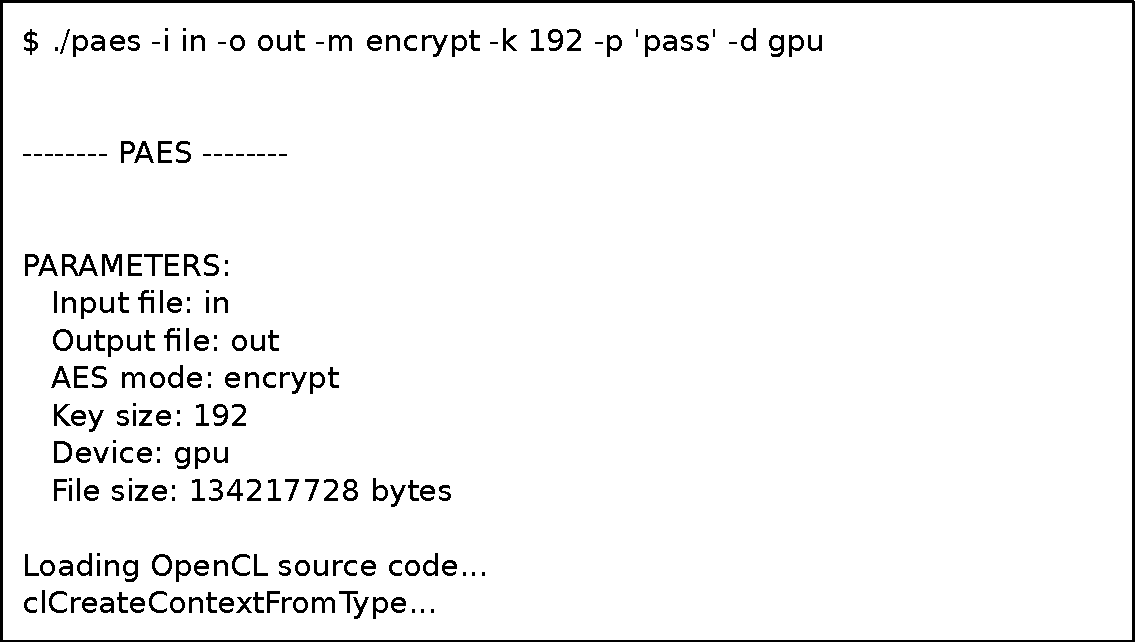
\includegraphics[width=\textwidth]{img/paes-screenshot}
\caption{PAES in azione.\label{fig:paes-screenshot}}
\end{center}
\end{figure}

\begin{table}[h]
\begin{center}
\begin{tabular}{|l|l|l|l|l|}
\hline
\textbf{Opzione} &  \textbf{Significato} \\
\hline
-i & file di input \\
\hline
-o & file di output \\
\hline
-m & modalità di uso di \ac{AES}, può essere \verb|encrypt| o \verb|decrypt| \\
\hline
-k & dimensione della chiave (\verb|128|, \verb|192| o \verb|256|) \\
\hline
-p & password usata per derivare la chiave per cifrare \\
\hline
-d & dispositivo da usare per il calcolo (\verb|cpu| o \verb|gpu|) \\
\hline
\end{tabular}
\caption{Opzioni della riga di comando di PAES.\label{tab:paes-opzioni}}
\end{center}
\end{table}

La gestione delle opzioni della riga di comando è stata implementata mediante la libreria \textit{getopt} abitualmente usata nei programmi Unix. In particolare, chiamate successive alla funzione \textit{getopt} restituiranno di volta in volta il carattere delle varie opzioni della riga di comando specificate dall'utente o -1 se non ve ne sono più; nella variabile \textit{optarg} è contenuto un puntatore all'eventuale valore dell'argomento associato all'opzione corrente. Oltre alle variabili \textit{argc} e \textit{argv}, che contengono gli argomenti separati e il loro numero, \textit{getopt} richiede un terzo argomento che consiste nella lista di lettere rappresentanti le varie opzioni, eventualmente seguite dai due punti qualora l'opzione richieda un argomento aggiuntivo. Il codice \ref{cod:paes-getopt} è un estratto del codice di PAES che mostra il semplicissimo utilizzo di \textit{getopt}.

\vspace*{10pt}
\begin{figure}
\begin{lstlisting}[caption={\textit{Lettura delle opzioni della riga di comando in PAES.}},label={cod:paes-getopt},language=C]
do {
	c = getopt(argc, argv, "hi:o:m:k:p:d:g:l:");	
	switch (c) {
		case 'i':
			*input_file_name = (char *) malloc(sizeof(char) * strlen(optarg) + 1);
			strcpy(*input_file_name, optarg);
			break;
		// ... similmente per le restanti opzioni
	}
} while (c != -1);
\end{lstlisting}
\end{figure}

\chapter{Implementazione}
\linespread{1}
\epigraph{\textit{One of my most productive days was throwing away 1000 lines of code.}}{K. Thompson}
\linespread{1.3}

\section{Programma host}

La componente di PAES in esecuzione sull'host si occupa di controllare le richieste dell'utente e preparare il device per l'esecuzione del compito desiderato. La lettura delle richieste lato utente avviene mediante la libreria \textit{getopt}, come descritto nella sezione \ref{sec:paes-cli}. Una volta letti i dati in input PAES controlla che questi abbiano senso: ad esempio il dispositivo da usare deve essere \verb|cpu| o \verb|gpu|, nessun'altro valore è ammissibile.

La password inserita dall'utente invece viene trattata in modo particolare; l'utente infatti può inserire parole chiave di lunghezza arbitraria, mentre \ac{AES} necessita di chiavi dalla lunghezza prefissata (128, 192 o 256 bit). Per questo motivo PAES calcola l'hash SHA-256 della password in questione: poiché questa funzione produce un hash di 256 bit è sempre possibile ricavare da quest'ultimo una chiave \ac{AES} di qualsiasi lunghezza ammissibile. La funzione SHA-256 utilizzata è stata ripresa dal codice di \ac{GnuPG}\footnote{http://www.gnupg.org/} e leggermente adattata per farla funzionare al di fuori del suo programma originario. Qualora l'utente non specifici la password mediante l'argomento della riga di comando \verb|-p| gli verrà richiesta interattivamente mediante la funzione \textit{getpass}: l'inserimento della password seguirà lo standard de facto in Unix, quindi a schermo non verrà visualizzato ciò che l'utente sta digitando ma alla pressione del tasto INVIO la password verrà memorizzata correttamente.

Successivamente PAES leggerà dal disco il contenuto del file da cifrare e richiamerà la funzione \textit{apply\_aes}, che si occuperà di preparare ed eseguire il programma \ac{OpenCL} sul dispositivo specificato. Il risultato di quest'ultima operazione verrà infine scritto nel file di output.

\subsection{La funzione apply\_aes}
\label{sec:paes-apply-aes}

Questa funzione, contenuta nel file \textit{paes\_functions.c} (vedi sezione \ref{sec:paes-files}), si occupa di preparare ed eseguire il programma \ac{OpenCL} sul dispositivo specificato dall'utente. Il processo è composto da una serie di passaggi piuttosto semplici, anche se tediosi, basati principalmente su chiamate \ac{API} di \ac{OpenCL}. Per ogni chiamata viene controllato se è stata eseguita con successo: in caso contrario l'esecuzione della funzione termina, rilasciando comunque tutti gli oggetti allocati fino a quel momento. Se tutte le chiamate vengono eseguite con successo, la funzione termina normalmente e la memoria allocata viene comunque liberata. Negli esempi di codice riportati di seguito le istruzioni per il controllo degli errori sono omesse per brevità e chiarezza.

Il primo passo consiste nel determinare l'implementazione di \ac{OpenCL} (definita con il sostantivo ``piattaforma'') che PAES dovrà utilizzare. Verrà sempre usata la prima implementazione trovata, in quanto in un'installazione realistica non vi saranno mai più piattaforme \ac{OpenCL} contemporaneamente onde evitare conflitti e potenziali problemi di compatibilità. Il codice \ref{cod:paes-platform} mostra le chiamate necessarie per determinare la piattaforma \ac{OpenCL} presente sulla macchina. Dalla piattaforma verrà poi ricavato il contesto nel quale eseguire i kernel \ac{OpenCL} (vedi sezione \ref{sec:opencl-code-contesti}). Si noti la necessità di effettuare una chiamata \ac{OpenCL} per controllare quante piattaforme sono effettivamente disponibili prima di allocare un'array per memorizzarle: questo modo di procedere è molto comune nell'\ac{API} \ac{OpenCL} ove sia necessario reperire informazioni di grandezza variabile da memorizzare nell'heap.

\begin{figure}
\begin{lstlisting}[caption={\textit{Scelta dell'implementazione di \ac{OpenCL} da utilizzare.}},label={cod:paes-platform},language=C]
clGetPlatformIDs(0, NULL, &num_platforms);
platforms = (cl_platform_id *) malloc(sizeof(cl_platform_id) * num_platforms);
clGetPlatformIDs(num_platforms, platforms, NULL);	
cl_context_properties cps[3] = {CL_CONTEXT_PLATFORM,
   (cl_context_properties)platforms[0], 0};
cl_context_properties *cprops;
if (NULL == platforms[0]) cprops = NULL;
else cprops = cps;
context = clCreateContextFromType(cprops, device_type[device], NULL, NULL, &error);
\end{lstlisting}
\end{figure}

Grazie al contesto è ora possibile selezionare il device sul quale eseguire effettivamente il calcolo. Sulla base dell'input dell'utente tale device può essere una \ac{GPU} o una \ac{CPU}; anche in questo caso viene selezionato il primo device della tipologia desiderata in quanto generalmente l'unico del genere presente sulla macchina (si noti che una \ac{CPU} multi-core è comunque vista come un'unica \ac{CPU} contenente più \ac{CU}). Questo processo è visibile nel codice di Figura \ref{cod:paes-device}. Anche in questo caso viene prima trovato il numero di dispositivi disponibili, poi vengono memorizzati i riferimenti agli stessi in un'array di lunghezza adeguata. Poiché verrà sempre usato il primo device trovato, d'ora in poi verrà sempre usato il primo elemento dell'array \textit{devices}, ovvero \textit{devices[0]}.

\begin{figure}
\begin{lstlisting}[caption={\textit{Selezione del device da utilizzare.}},label={cod:paes-device},language=C]
size_t context_information_size;
clGetContextInfo(context, CL_CONTEXT_DEVICES, 0, NULL,
    &context_information_size);
devices = (cl_device_id *) malloc(context_information_size);
clGetContextInfo(context, CL_CONTEXT_DEVICES, context_information_size, devices, NULL);
\end{lstlisting}
\end{figure}

Una volta trovato il dispositivo si può creare una coda dei comandi associata allo stesso come descritto nel codice \ref{cod:paes-create-queue}. È fondamentale specificare il parametro \textit{CL\_QUEUE\_PROFILING\_ENABLE} che consente di abilitare la misura dei tempi di esecuzione dei comandi eseguiti nella coda appena creata.

\begin{figure}
\begin{lstlisting}[caption={\textit{Creazione di una coda di comandi.}},label={cod:paes-create-queue},language=C]
clCreateCommandQueue(context, devices[0], CL_QUEUE_PROFILING_ENABLE, &error);
\end{lstlisting}
\end{figure}

Poiché \ac{AES} richiede che la chiave ricavata dalla password dell'utente venga espansa per generare le diverse sottochiavi, è necessario procedere con questa operazione (vedi codice \ref{cod:paes-keyexpansion}). Poiché la creazione delle sottochiavi ha un costo molto piccolo e indipendente dalla dimensione dei dati in ingresso questo calcolo viene svolto direttamente dal programma host per evitare inutili complicazioni. Il comportamento delle funzioni \textit{get\_round\_key\_size} e \textit{key\_expansion} ricalca perfettamente quanto riportato nello standard \ac{AES} ed è stato già descritto nella sezione \ref{sec:aes-key-schedule}.

\begin{figure}
\begin{lstlisting}[caption={\textit{Creazione delle sottochiavi \ac{AES}.}},label={cod:paes-keyexpansion},language=C]
cl_uint round_key_size = get_round_key_size(key_size_bits);
cl_uchar *round_key = key_expansion(key, key_size_bits);
\end{lstlisting}
\end{figure}

A questo punto è necessario scrivere nella memoria del dispositivo di calcolo i dati su cui dovrà essere applicato \ac{AES}. Prima di tutto si crea un buffer \ac{OpenCL} mediante la chiamata \textit{clCreateBuffer}; il buffer viene creato in modalità lettura e scrittura poiché servirà anche per contenere il risultato della computazione. Quindi, tramite la funzione \textit{clEnqueueWriteBuffer}, viene messa nella coda dei comandi un'istruzione per la scrittura del buffer nella memoria del device; all'operazione di scrittura viene associato un evento che servirà in seguito per misurare le prestazioni. Il terzo parametro di questa chiamata indica che l'operazione è bloccante, quindi il flusso del programma host rimarrà fermo fino al suo completamento. Le operazioni illustrate in questo paragrafo sono implementate dal codice \ref{cod:paes-write-buffer}.

\begin{figure}
\begin{lstlisting}[caption={\textit{Creazione e scrittura del buffer nella memoria del dispositivo.}},label={cod:paes-write-buffer},language=C]
cl_buffer = clCreateBuffer(context, CL_MEM_READ_WRITE,
   sizeof(cl_uchar) * size, NULL, &error);
clEnqueueWriteBuffer(command_queue, cl_buffer, CL_TRUE, 0, 
   sizeof(cl_uchar) * size, (void *) buffer, 0, NULL,
   &event_write);
\end{lstlisting}
\end{figure}

Il programma \ac{OpenCL} deve essere compilato per il device in cui verrà eseguito. Purtroppo al momento della stesura l'implementazione \ac{OpenCL} di AMD non supporta il caricamento di file binari compilati in precedenza, quindi è necessario compilare il sorgente \ac{OpenCL} sul momento. Il codice \ref{cod:paes-compile} mostra le istruzioni necessarie per la compilazione del sorgente: il codice del programma \ac{OpenCL} è contenuto nella variabile \textit{source}, di dimensione \textit{source\_size}, che è stata caricata in precedenza con il contenuto del file sorgente \textit{paes.cl} (vedi sezione \ref{sec:paes-files}).

\begin{figure}
\begin{lstlisting}[caption={\textit{Compilazione del programma da eseguire sul dispositivo.}},label={cod:paes-compile},language=C]
program = clCreateProgramWithSource(context, 1,
   (const char **) &source, &source_size, &error);
clBuildProgram(program, 0, NULL, NULL, NULL, NULL);
clGetProgramBuildInfo(program, devices[0], CL_PROGRAM_BUILD_LOG, 300, build_log, NULL);
printf("\nBuild log:\n%s\n", build_log);
\end{lstlisting}
\end{figure}

Avendo a disposizione il programma compilato, grazie alla funzione \textit{clCreateKernel} è possibile selezionare il codice binario del kernel che verrà eseguito nel device. Il codice \ref{cod:paes-compile} mostra come creare un oggetto kernel che verrà usato per eseguire la computazione nonché il modo per impostare gli argomenti che rimarranno fissi durante la stessa grazie alla funzione \textit{clSetKernelArg}. Alcune note importati su quest'ultima operazione:
\begin{enumerate}
\item Gli argomenti per il kernel destinati a essere memorizzati nella Global Memory o nella Constant Memory necessitano di un apposito buffer \ac{OpenCL} e sarà quest'ultimo a essere usato come argomento; poiché per le sottochiavi non era ancora stato creato un buffer è necessario farlo ora. Questo buffer è impostato in modalità sola lettura in quanto durante la computazione non è mai necessario scrivervi.
\item Gli argomenti che verranno salvati nella Private Memory possono invece essere passati senza ricorrere a buffer intermedi.
\item \textit{clSetKernelArg} richiede che venga specificato l'indice dell'argomento da passare; tale indice parte da 0 e ricalca fedelmente l'ordine degli argomenti della funzione kernel.
\end{enumerate}
La creazione del kernel e l'impostazione degli argomenti fissi è implementata dal codice \ref{cod:paes-set-args}; il nome del kernel ovviamente deve essere lo stesso di quello dichiarato nel sorgente \ac{OpenCL} (vedi sezione \ref{sec:paes-kernel}).

\begin{figure}
\begin{lstlisting}[caption={\textit{Creazione del kernel e impostazione degli argomenti fissi.}},label={cod:paes-set-args},language=C]
clCreateKernel(program, "kernel_aes", &error);

clSetKernelArg(kernel, 0, sizeof(cl_mem), (void *) &cl_buffer);
clSetKernelArg(kernel, 1, sizeof(cl_ulong), (void *) &blocks);
clSetKernelArg(kernel, 2, sizeof(cl_uint), (void *) &mode);

cl_rkey = clCreateBuffer(context,
   CL_MEM_READ_ONLY | CL_MEM_USE_HOST_PTR,
   sizeof(cl_uchar) * round_key_size, round_key, &error2);
clSetKernelArg(kernel, 3, sizeof(cl_mem), (void *) &cl_rkey);

clSetKernelArg(kernel, 4, sizeof(cl_uint), (void *) &rounds);
\end{lstlisting}
\end{figure}

Il codice \ref{cod:paes-run} mostra infine l'esecuzione del kernel. Il kernel in questione esegue soltanto un round \ac{AES} specificato in un parametro impostato nel programma host; tale parametro deve quindi essere cambiato di volta in volta, a differenza di quelli impostati precedentemente che rimangono fissi. Il kernel viene eseguito sullo spazio degli indici definiti da \textit{global\_size} e \textit{local\_size}; il metodo per determinare tali valori è descritto nella sezione \ref{subsec:paes-global-local-size}. Mettere in coda l'esecuzione del kernel non è un'operazione bloccante quindi è necessario ricorrere alla chiamata \textit{clFinish} per sincronizzare il programma host con quello eseguito sul device. I tempi di esecuzione dei vari round vengono sommati per ottenere il tempo totale impiegato per la cifratura \ac{AES}.

\begin{figure}
\begin{lstlisting}[caption={\textit{Esecuzione del kernel.}},label={cod:paes-run},language=C]
double execution_time = 0;
for (cl_uint round = 0; round <= rounds; ++round) {
	clSetKernelArg(kernel, 5, sizeof(cl_uint), (void *) &round);		
	
	clEnqueueNDRangeKernel(command_queue, kernel, 1, NULL, 
		&global_size, &local_size, 0, NULL, &event_execute);
	clFinish(command_queue);
	
	execution_time += execution_time_msecs(event_execute);
}
\end{lstlisting}
\end{figure}

Per ottenere il risultato della computazione è necessaria ancora un'altra istruzione per la coda dei comandi del device, descritta nel codice di Figura \ref{cod:paes-read-clean}. L'istruzione è anch'essa bloccante e viene associata a un evento per misurarne il tempo d'esecuzione.

È infine fondamentale rilasciare scrupolosamente tutti gli oggetti allocati nel corso di questa lunga serie di operazioni per evitare che la macchina e i device utilizzati vengano saturati nel corso di esecuzioni successive del programma; a tale scopo, oltre alla consueta istruzione \textit{free}, \ac{OpenCL} mette a disposizione una serie di chiamate \ac{API} per deallocare le varie tipologie di oggetti specifiche di \ac{OpenCL} stesso. Nel caso di PAES sono necessarie rispettivamente \textit{clReleaseEvent}, \textit{clReleaseMemObject}, \textit{clReleaseKernel}, \textit{clReleaseProgram}, \textit{clReleaseCommandQueue} e \textit{clReleaseContext}.

\begin{figure}
\begin{lstlisting}[caption={\textit{Lettura del risultato dell'esecuzione del kernel.}},label={cod:paes-read-clean},language=C]
clEnqueueReadBuffer(command_queue, cl_buffer, CL_TRUE, 0, sizeof(cl_uchar) * size, buffer, 0, NULL, &event_read);
\end{lstlisting}
\end{figure}

\subsection{Global e local size}
\label{subsec:paes-global-local-size}

PAES consente di gestire global e local size in due modi:
\begin{enumerate}
\item staticamente;
\item dinamicamente.
\end{enumerate}

L'uso di un file header dedicato (in questo caso \textit{paes\_size.h}) rende possibile la scrittura di politiche dinamiche per determinare global e local size in base alla dimensione dell'input. Nel file possono essere contenuti i seguenti valori:
\begin{description}
\item[PAES\_DYNAMIC\_SIZE:] se definito, abilita la politica dinamica;
\item[PAES\_MAX\_LOCAL\_SIZE:] il massimo valore da assegnare alla local size;
\item[PAES\_GLOBAL\_LOCAL\_RATIO:] il rapporto tra global e local size.
\end{description}

PAES cerca di impostare una global size pari al numero di blocchi \ac{AES} del file da cifrare mentre la local size è ottenuta come rapporto tra global e local size. Qualora il numero di workgroup, ovvero $\frac{global\_size}{local\_size}$, superi i limiti fisici del device, la global size viene ridimensionata.

Se invece si desidera usare valori fissi per local e global size bisogna impostare le seguenti costanti simboliche nel file header:
\begin{description}
\item[PAES\_STATIC\_SIZE:] se definito, abilita la politica statica;
\item[PAES\_LOCAL\_SIZE:] il valore da assegnare alla local size;
\item[PAES\_GLOBAL\_SIZE:] il valora da essegnare alla global size.
\end{description}

\subsection{Misura delle prestazioni}

Le prestazioni del programma eseguito sul dispositivo \ac{OpenCL} vengono misurate mediante gli eventi messi a disposizione da \ac{OpenCL} stesso. Dato un evento associato a un comando della coda di esecuzione terminato correttamente, è possibile risalire al tempo di esecuzione del comando stesso mediante la semplice funzione riportata nel codice di Figura \ref{cod:paes-event}.

\begin{figure}
\begin{lstlisting}[caption={\textit{Misura delle prestazioni di un comando tramite eventi.}},label={cod:paes-event},language=C]
static double execution_time_msecs(cl_event event)
{
	cl_ulong start, end;
	clGetEventProfilingInfo(event, CL_PROFILING_COMMAND_START, sizeof(cl_ulong), &start, NULL);
	clGetEventProfilingInfo(event, CL_PROFILING_COMMAND_END, sizeof(cl_ulong), &end, NULL);
	return (end - start) * 1.0E-6;
}
\end{lstlisting}
\end{figure}

L'esecuzione viene misurata con una risoluzione nell'ordine teorico dei nanosecondi, ma per gli scopi di PAES il valore viene riportato in millisecondi per fornire una misura più chiara e comunque assolutamente significativa.

\section{Kernel}
\label{sec:paes-kernel}

Come visto nella sezione \ref{sec:paes-files} il kernel \ac{OpenCL} di PAES e le funzioni da esso utilizzate sono contenute nel file \textit{paes.cl}. La funzione kernel, richiamata dal programma host, ha il prototipo riportato nel codice di Figura \ref{cod:paes-kernel}.

\begin{figure}
\begin{lstlisting}[caption={\textit{Prototipo del kernel di PAES.}},label={cod:paes-kernel},language=C]
__kernel __attribute__ ((vec_type_hint(uchar)))
void kernel_aes(
	__global uchar16 *buffer, 
	const ulong blocks, 
	const uint mode, 
	__constant const uchar16 *round_key, 
	const uint rounds, 
	const uint round)
\end{lstlisting}
\end{figure}

Come da standard, il prototipo deve iniziare con il qualificatore \verb|__kernel|. Il qualificatore \verb|__attribute__| e il suo argomento sono definiti dallo standard in questo modo:
\begin{quotation}
\textit{\_\_attribute\_\_((vec\_type\_hint(<type>))) è un suggerimento opzionale per il compilatore; serve a rappresentare la larghezza computazionale della funzione kernel e dovrebbe servire come base per il calcolo dell'uso della larghezza di banda del processore quando il compilatore sta cercando di autovettorizzare il codice.}\cite{bib:opencl}
\end{quotation}

I parametri del kernel hanno questo significato:
\begin{description}
\item[\textit{buffer}:] il vettore contenente i blocchi da cifrare, che verranno sovrascritti coi blocchi cifrati, allocati nella Global Memory;
\item[\textit{blocks}:] il numero di blocchi \ac{AES} contenuti nel buffer;
\item[\textit{mode}:] indica se si vuole cifrare o decifrare i dati;
\item[\textit{round\_key}:] le sottochiavi, allocate nella Constant Memory;
\item[\textit{rounds}:] il numero totale di round previsto per la lunghezza di chiave selezionata dall'utente;
\item[\textit{round}:] il round che il kernel deve eseguire.
\end{description}

Il buffer, passato dal programma host come array di singoli \textit{char} privi di segno viene qui rappresentato come array di \textit{uchar16}: si tratta di un tipo vettoriale di \ac{OpenCL} contenente 16 byte, ovvero proprio la dimensione di un blocco \ac{AES}. Il cambio di rappresentazione non inficia la corretta lettura dei valori nel buffer in quanto in layout dei dati in memoria rimane identico; d'altro canto l'uso di \textit{uchar16} consente di semplificare la scrittura del codice \ac{AES} rendendolo più comprensibile, sia per la mappatura diretta dei blocchi sia per alcune peculiarità dei tipi vettoriali \ac{OpenCL} che saranno descritte in seguito.

\begin{figure}
\begin{lstlisting}[caption={\textit{Selezione dei blocchi per ciascun work-item.}},label={cod:paes-blocks},language=C]
size_t global_work_size = get_global_size(0);
size_t global_id = get_global_id(0);

size_t blocks_per_work_item;
if (global_work_size < blocks)
	blocks_per_work_item = blocks / global_work_size;
else
	blocks_per_work_item = 1;

size_t reminder;
if (global_work_size < blocks)
	reminder = blocks % global_work_size;
else
	reminder = 0;

size_t from_block = global_id * blocks_per_work_item;
if (global_id < reminder) 
	from_block += global_id;
else 
	from_block += reminder;
\end{lstlisting}
\end{figure}

Prima di tutto ciascuna istanza del kernel calcola l'intervallo di blocchi del buffer di input che dovrà cifrare. Il calcolo, descritto nel codice di Figura \ref{cod:paes-blocks} implementa la logica descritta nella sezione \ref{sec:paes-parallelism} che, ricordo, ripartisce uniformemente i blocchi da cifrare tra i work-item disponibili.

\begin{figure}
\begin{lstlisting}[caption={\textit{Codice principale del kernel.}},label={cod:paes-kernel-main},language=C]
if (from_block < blocks) {
	size_t to_block = from_block + blocks_per_work_item;	
	if (global_id < reminder) 
		to_block += 1;

	if (mode == AES_MODE_ENCRYPT)
	    for (size_t b = from_block; b < to_block; ++b)
            // Cifra il blocco buffer[b]
    else
	    for (size_t b = from_block; b < to_block; ++b)
            // Decifra il blocco buffer[b]
}
\end{lstlisting}
\end{figure}

A questo punto il work-item ha tutte le informazioni necessarie per svolgere la sua parte di computazione, il cui schema è riportato nel codice di Figura \ref{cod:paes-kernel-main}. Innanzitutto ciascuna istanza del kernel controlla se deve effettivamente cifrare dei blocchi (qualora \textit{global\_worksize} $<$ \textit{blocks}, alcuni work-item non devono fare nulla); se questo è il caso, \ac{AES} è applicato a tutti i blocchi di propria competenza.

\begin{figure}
\begin{lstlisting}[caption={\textit{Codice kernel per la cifratura di un blocco.}},label={cod:paes-encrypt},language=C]
#ifdef SHIFT_ROWS
	shift_rows(b, buffer);
#elif defined(MIX_COLUMNS)
	mix_columns(b, buffer);
#elif defined(ADD_ROUND_KEY)
	buffer[b] ^= round_key[rounds];
#elif defined(SUB_BYTES)
	sub_bytes(b, buffer, sbox_encrypt);
#else
	if (round == 0) {
		buffer[b] ^= round_key[0];
	} else if (round == rounds) {
		sub_bytes(b, buffer, sbox_encrypt);
		shift_rows(b, buffer);
		buffer[b] ^= round_key[rounds];
	} else {
		sub_bytes(b, buffer, sbox_encrypt);
		shift_rows(b, buffer);
		mix_columns(b, buffer);
		buffer[b] ^= round_key[round];
	}
#endif
\end{lstlisting}
\end{figure}

Il codice del kernel per cifrare un blocco è riportato nel codice di Figura \ref{cod:paes-encrypt}, quello per decifrare è molto simile. Le istruzioni condizionali del preprocessore vengono usate nella compilazione in fase di test (vedi sezione \ref{sec:test}) allo scopo di consentire controlli sulla conformità allo standard delle singole funzioni \ac{AES}; normalmente verrà sempre compilato il codice contenuto nel ramo \textit{\#else}, che in effetti implementa un singolo round \ac{AES} con gli opportuni accorgimenti per il primo e l'ultimo round.

Le primitive \ac{AES} sono implementate come funzioni all'interno del medesimo sorgente \ac{OpenCL}, con l'esclusione della \textit{AddRoundKey} che è rappresentabile da una singola istruzione; questo perché l'uso dei tipi di dato vettoriali \ac{OpenCL} consente l'applicazione di operazioni a tutti gli elementi del vettore contemporaneamente (in questo caso, l'\textit{or} esclusivo).

\begin{figure}
\begin{lstlisting}[caption={\textit{Funzione SubBytes definita nel kernel.}},label={cod:paes-subbytes},language=C]
__constant const uchar sbox_encrypt[256] = AES_SBOX_ENCRYPT;
__constant const uchar sbox_decrypt[256] = AES_SBOX_DECRYPT;

void sub_bytes(size_t block, __global uchar16 *buffer, __constant const uchar *sbox)
{
	buffer[block] = (uchar16)(sbox[buffer[block][0]], 
								sbox[buffer[block][1]],
								sbox[buffer[block][2]], 
								sbox[buffer[block][3]], 
								// ... 
								sbox[buffer[block][13]], 
								sbox[buffer[block][14]],
								sbox[buffer[block][15]]);
}
\end{lstlisting}
\end{figure}

Come esempio delle restanti funzioni \ac{AES}, il codice \ref{cod:paes-subbytes} riporta la \ac{S-box}. Il parametro \textit{block}, ovvero il blocco su cui lavorare, e \textit{buffer}, corrispondente al \textit{buffer} di input/output della funzione kernel, sono comuni a tutte le primitive \ac{AES}; la tabella usata per contenere i valori di tutte le sostituzioni possibili, una peculiarità della funzione \textit{sub\_bytes}, è invece un puntatore a un'area della Constant Memory allocata con una costante globale nel codice sorgente \ac{OpenCL}.

Anche in questo caso viene sfruttata una sintassi peculiare dei tipi vettoriali \ac{OpenCL}, il costruttore anonimo; i singoli elementi del risultato sono ottenuti con la sostituzione mediante la tabella che rappresenta la \ac{S-box}. Poiché tale tabella è un parametro, la funzione \textit{sub\_bytes} può essere usata sia per cifrare che per decifrare semplicemente cambiando quest'ultimo.

\chapter{Metodologia}
\linespread{1}
\epigraph{\textit{Though this be madness, yet there is method in't.}}{W. Shakespeare}
\linespread{1.3}

Poiché lo scopo principale di PAES era quello di esplorare l'uso di \ac{OpenCL} è stata posta particolare attenzione alla metodologia usata e alle sue differenze e somiglianze rispetto a quella canonica per lo sviluppo di programmi C.

\ac{OpenCL} è uno standard ben definito, tuttavia le sue implementazioni sono ancora piuttosto instabili. Per questo motivo è stato opportuno isolare le chiamate \ac{OpenCL} all'interno di una procedura (in questo caso si tratta di \textit{apply\_aes}, descritta nella sezione \ref{sec:paes-apply-aes}); in questo modo si limita l'impatto dei problemi delle implementazioni \ac{OpenCL} a una parte di codice molto ben definita.

Il resto del programma host è quasi completamente svincolato dalle idiosincrasie di \ac{OpenCL} salvo che per un punto fondamentale: i tipi di dato. Infatti la dimensione dei tipi di dato standard del linguaggio C (es. \textit{int}) può variare tra l'host e il particolare device usato; a questo scopo \ac{OpenCL} definisce dei tipi di dato da utilizzare al posto di quelli standard la cui dimensione è garantita essere identica sia nell'host che nei device. Ad esempio in PAES l'input è rappresentato come un vettore di tipo \textit{cl\_uchar}, il corrispettivo \ac{OpenCL} del tipo \textit{unsigned char}.

Dato che \ac{OpenCL} consente di eseguire programmi su device assolutamente eterogenei, PAES è stato strutturato in modo da avere la maggior libertà possibile nella scelta di local e global size (vedi sezione \ref{sec:paes-parallelism}); l'uso di un file header dedicato per questi valori (vedi sottosezione \ref{subsec:paes-global-local-size}) consente di averne più copie pronte per l'uso, ciascuna ottimizzata per un particolare dispositivo.

Sebbene il programma per il device sia scritto in un linguaggio con alcune limitazioni rispetto al C standard (vedi sezione \ref{sec:opencl-c99}) è stato opportuno evitare la duplicazione di definizioni di costanti e tipi di dato tra il programma host e quello per il device: a questo scopo è stato creato il file \textit{paes\_constants\_and\_datatypes.h}. Poiché il dialetto C \ac{OpenCL} non supporta l'uso delle enumerazioni è stato necessario usare la direttiva del preprocessore \textit{\#define} per la definizione di valori costanti; in questo caso è stato scelto un compromesso tra minor duplicazione del codice e maggior pericolo di inconsistenze dei tipi di dato.

PAES è stato strutturato in maniera da poter essere usato in modo pressoché indolore da altri programmi. In effetti per riutilizzare il codice di PAES è sufficiente richiamare la funzione \textit{apply\_aes}, per il cui funzionamento sono necessari i file \textit{paes.cl}, \textit{paes\_constants\_and\_datatypes.h}, \textit{paes\_size.h}, \textit{paes\_functions.h} e \textit{paes\_functions.c}. Sempre nell'ottica di favorire il riuso del codice tutte le funzioni, i tipi di dato e le costanti sono state ampiamente documentate.

\section{Automazione dei test}
\label{sec:test}
Durante lo sviluppo di PAES è stato fondamentale valutarne sia la correttezza che le prestazioni.

Lo sviluppo dei test per la conformità rispetto allo standard \ac{AES} e per la misura delle prestazioni è iniziato parallelamente rispetto a quello del nucleo di PAES; lungi dall'essere un peso, infatti, questo modo di procedere agevola il lavoro complessivo da svolgere rendendo più semplice mantenere sotto controllo la complessità del codice che, inevitabilmente, cresce col passare del tempo \cite{bib:test}.

Come riferimento per i test, sia di correttezza che di prestazioni, è stata selezionata un'implementazione seriale di \ac{AES} corretta il cui codice è di facile comprensione, a patto che si conosca bene il funzionamento di \ac{AES}.

I test sono implementati mediante script Python; oltre a essere portabili come e più di PAES, ciò li rende anche facilmente modificabili. In questo modo si è evitato di rendere pesante l'aggiornamento dei test parallelamente con la crescita di PAES, cosa che avrebbe potuto disincentivarlo completamente.

Tutti i test di PAES sono implementati mediante discendenti della classe \textit{BaseTest}. Qui sono definiti una serie di metodi di utilità generale (vedi tabella \ref{tab:paes-basetest}) che verranno poi usati dalle sottoclassi. In particolare i discendenti dovranno implementare gli specifici test da eseguire nel metodo \textit{test} e richiamare il metodo \textit{run} nel codice principale dello script.

Grazie a \textit{BaseTest} tutti i test vengono eseguiti in directory temporanee: se il test ha successo la sua directory temporanea viene cancellata, altrimenti rimane sul disco, a disposizione per ulteriori indagini. Inoltre \textit{BaseTest} fornisce alle sottoclassi i metodi per la scrittura di un file di log dal formato predefinito con tutte le informazioni necessarie per contestualizzare i risultati di un test (nome del test, nome host, device utilizzato, durata\ldots{}).

\begin{table}[h]
\begin{center}
\begin{tabular}{|l|l|l|l|l|}
\hline
\textbf{Metodo} &  \textbf{Descrizione} \\
\hline
\textit{compile\_paes(opt)} & compila PAES e prepara l'ambiente per eseguirlo \\
\hline
\textit{compile\_aes(opt)} & compila l'\ac{AES} di riferimento \\
\hline
\textit{cleanup} & elimina la directory temporanea del test \\
\hline
\textit{create\_dummy(size)} & crea un file casuale di dimensione \textit{size} \\
\hline
\textit{paes(opt)} & esegue PAES con le opzioni specificate \\
\hline
\textit{aes(opt)} & esegue l'\ac{AES} di riferimento con le opzioni specificate \\
\hline
\textit{diff(f1, f2)} & controlla se i due file \textit{f1} e \textit{f2} sono uguali \\
\hline
\textit{echo(msg)} & scrive su un file di log il messaggio specificato \\
\hline
\end{tabular}
\caption{Principali metodi della classe BaseTest.\label{tab:paes-basetest}}
\end{center}
\end{table}

I test che sono stati effettivamente implementati sfruttando questa infrastruttura sono:
\begin{description}
\item[TestBijectivity:] controlla che l'implementazione di PAES sia biettiva, ovvero l'applicazione della procedura di cifratura prima e di decifratura poi a un input qualsiasi dovrebbe produrre un risultato identico all'input stesso; ovviamente non si tratta di un test di correttezza ma di un metodo semplice e veloce per rilevare errori grossolani.
\item[TestConformance:] controlla che PAES produca gli stessi risultati dell'implementazione \ac{AES} di riferimento, sia globalmente sia a livello delle singole operazioni \ac{AES} (\textit{SubBytes}, \textit{ShiftRows}, \textit{MixColumns}, \textit{AddRoundKey}); il tutto sia per la cifratura che per la decifratura.
\item[TestPerformance:] rileva le prestazioni di PAES per una serie di file di dimensione crescente; le rilevazioni sono fatte sia per la cifratura che per la decifratura nonché per le operazioni di lettura e scrittura verso il device.
\end{description}

\chapter{Valutazione delle prestazioni}
\linespread{1}
\epigraph{\textit{Software is getting slower more rapidly than hardware becomes faster.}}{N. Wirth}
\linespread{1.3}

Le analisi delle prestazioni di PAES sono state svolte, sia per quanto riguarda la versione \ac{OpenCL} su \ac{CPU} che per quella seriale, su un processore Intel Dual Core, avente le caratteristiche seguenti:
\begin{verbatim}
Name: Intel(R) Core(TM)2 CPU 6300 @ 1.86GHz (64 bit)
Vendor: GenuineIntel
Max compute units: 2
Max work item sizes: [1024, 1024, 1024]
Max work group size: 1024
Max clock frequency: 1.86 GHz
Max memory allocation size: 1 Gb
Global memory size: 3 Gb
Max constant buffer size: 64 Kb
Max constant arguments: 8
Local memory size: 32 Kb
\end{verbatim}

I test su \ac{GPU} invece si sono avvalsi di una scheda grafica GeForce GTX 275, le cui caratteristiche principali sono:
\begin{verbatim}
Name: GeForce GTX 275 (32 bit)
Vendor: NVIDIA Corporation
Max compute units: 30
Max work item sizes: [512, 512, 64]
Max work group size: 512
Max clock frequency: 1.40 GHz
Max memory allocation size: 223 Mb
Global memory size: 895 Mb
Max constant buffer size: 64 Kb
Max constant arguments: 9
Local memory size: 16 Kb
\end{verbatim}

Queste caratteristiche sono state rilevate mediante un semplice programma diagnostico che sfrutta una serie di chiamate \ac{API} \ac{OpenCL} per interrogare i device; i dati riportati sopra sono il risultato della sua esecuzione sui due device.

Si noti come la \ac{CPU} abbia soltanto 2 core operanti in modalità a 64 bit, rispetto alle 30 \ac{CU} a 32 bit della \ac{GPU}; tuttavia quest'ultime sono piuttosto specializzate per programmi che sfruttano il paradigma \ac{SIMD} o \ac{SPMD} mentre le unità di calcolo della \ac{CPU} sono state concepite per un uso più generale. La frequenza dei core della \ac{CPU} è leggermente superiore a quella delle \ac{CU} della \ac{GPU}.

Il parametro \verb|Global memory size| indica la quantità di Global Memory disponibile per un singolo kernel:  la dotazione della \ac{CPU} è decisamente migliore rispetto a quella della \ac{GPU}. Un altro parametro interessante è la dimensione massima per l'allocazione di una singola variabile: la \ac{GPU} è limitata a 223 Mb, perciò i test riportati di seguito si limiteranno al raggiungimento di questa soglia.

Anche in ambito software la scelta di questi due device ha determinato una notevole eterogeneità: i test su \ac{CPU} si sono necessariamente avvalsi dell'implementazione \ac{OpenCL} di AMD mentre per la \ac{GPU} è stata usata quella della NVIDIA Corporation (vedi sezione \ref{sec:opencl-impl}).

\section{Input/output}

I test di banda riguardano le operazioni di lettura e scrittura nella Global Memory, sia della \ac{CPU} che della \ac{GPU}; ovviamente non hanno alcun senso per il programma seriale, basato su un modello di programmazione differente.

La dimensione della chiave \ac{AES} non influisce sulle operazioni di scrittura dei dati da cifrare nella Global Memory del device né sulla successiva lettura del risultato.

Le tabelle \ref{tab:test-read} e \ref{tab:test-write} riportano i risultati dei test rispettivamente in lettura e scrittura. È evidente che il costo sia della lettura che della scrittura è pressoché esponenziale rispetto alla grandezza dei dati da cifrare: si tratta di un overhead che non è possibile eliminare mediante artifici a livello di scrittura del codice sorgente \ac{OpenCL}. Nei grafici \ref{fig:test-read-cpu} e \ref{fig:test-write-cpu} sono rappresentati i risultati dei test su \ac{CPU} mentre quelli su \ac{GPU} sono nei grafici \ref{fig:test-read-gpu} e \ref{fig:test-write-gpu}.

\section{AES}

I test prestazionali più importanti sono sicuramente quelli che coinvolgono il codice che implementa \ac{AES}. I rilevamenti sono stati effettuati per la versione seriale e quella \ac{OpenCL} (sia su \ac{CPU} che su \ac{GPU}), per ciascuna lunghezza di chiave, sia per la cifratura che per la decifratura. I dati riportati nella tabella \ref{tab:test-encrypt} e rappresentati nel grafico \ref{fig:test-encrypt} sono una sintesi dei risultati dei test basata su questi due criteri:
\begin{enumerate}
\item sia la cifratura che la decifratura hanno lo stesso andamento in quanto le operazioni da svolgere sono del tutto simili;
\item le tre lunghezze di chiave \ac{AES} aumentano il numero di round allo stesso modo per tutte le implementazioni; pertanto, fissata la scelta tra \ac{AES} seriale o PAES su \ac{CPU} o \ac{GPU} la lunghezza della chiave non influisce sull'andamento dei risultati.
\end{enumerate}

Per il primo motivo sono riportati soltanto i risultati della cifratura, mentre per il secondo sono stati aggregati tramite media aritmetica i rilevamenti di ciascuna implementazione per tutte e tre le lunghezze di chiave.

Le tradizionali misure basate sullo speed-up non sono applicabili, in generale, per due motivi:
\begin{enumerate}
\item \ac{OpenCL} non consente di controllare direttamente il numero di unità di calcolo che il programma può usare;
\item il programma è stato eseguito su dispositivi eterogenei.
\end{enumerate}

Per dare un'idea dei rapporti tra le prestazioni delle varie implementazioni, nella tabella \ref{tab:test-ratio} sono riportate tre misure:
\begin{enumerate}
\item il rapporto dei tempi d'esecuzione tra le versioni \ac{OpenCL} su \ac{CPU} e \ac{GPU};
\item il rapporto dei tempi d'esecuzione tra la versione seriale e quella \ac{OpenCL} su \ac{GPU};
\item il rapporto dei tempi d'esecuzione tra la versione seriale e quella \ac{OpenCL} su \ac{CPU};
\end{enumerate}

Sulla base di questi indici è possibile fare alcune osservazioni; ad esempio:
\begin{enumerate}
\item PAES su \ac{CPU} è sempre più veloce del programma seriale;
\item PAES su \ac{GPU} è più veloce del programma seriale a partire da input di dimensione 512 Kb;
\item PAES su \ac{GPU} è più veloce di PAES su \ac{CPU} a partire da input di 8 Mb.
\end{enumerate}

In generale, all'aumentare della dimensione dei dati da cifrare, PAES su \ac{GPU} è la versione più performante; per input di piccole dimensioni invece l'overhead dovuto alle operazioni di lettura e scrittura sulla memoria della \ac{GPU} supera il guadagno nei tempi di calcolo.

\begin{table}[p]
\begin{center}
\begin{tabular}{|r|r|r|}
\hline
\textbf{Dimensione (byte)} & \textbf{CPU (ms)} & \textbf{GPU (ms)} \\
\hline
128 & 0.000 & 0.003 \\
\hline
256 & 0.001 & 0.003 \\
\hline
512 & 0.001 & 0.003 \\
\hline
1024 & 0.001 & 0.004 \\
\hline
2048 & 0.002 & 0.004 \\
\hline
4096 & 0.002 & 0.005 \\
\hline
8192 & 0.007 & 0.007 \\
\hline
16384 & 0.015 & 0.010 \\
\hline
32768 & 0.032 & 0.017 \\
\hline
65536 & 0.060 & 0.030 \\
\hline
131072 & 0.122 & 0.108 \\
\hline
262144 & 0.237 & 0.202 \\
\hline
524288 & 0.466 & 0.387 \\
\hline
1048576 & 1.147 & 0.774 \\
\hline
2097152 & 2.433 & 1.172 \\
\hline
4194304 & 4.716 & 2.001 \\
\hline
8388608 & 9.434 & 3.593 \\
\hline
16777216 & 18.621 & 6.892 \\
\hline
33554432 & 37.023 & 13.436 \\
\hline
67108864 & 73.977 & 26.475 \\
\hline
134217728 & 162.418 & 52.453 \\
\hline
234700800 & 267.740 & 91.343 \\
\hline
\end{tabular}
\caption{Tempi di lettura dalla Global Memory.\label{tab:test-read}}
\end{center}
\end{table}

\begin{figure}[p]
\begin{center}
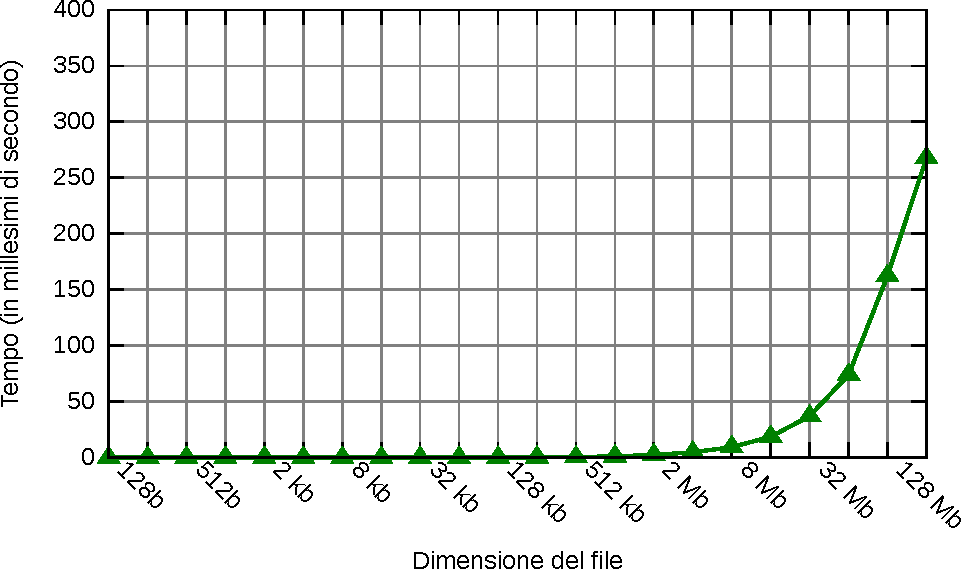
\includegraphics[width=\textwidth]{img/test-read-cpu}
\caption{Tempi di lettura dalla Global Memory della CPU.\label{fig:test-read-cpu}}
\end{center}
\end{figure}

\begin{figure}[p]
\begin{center}
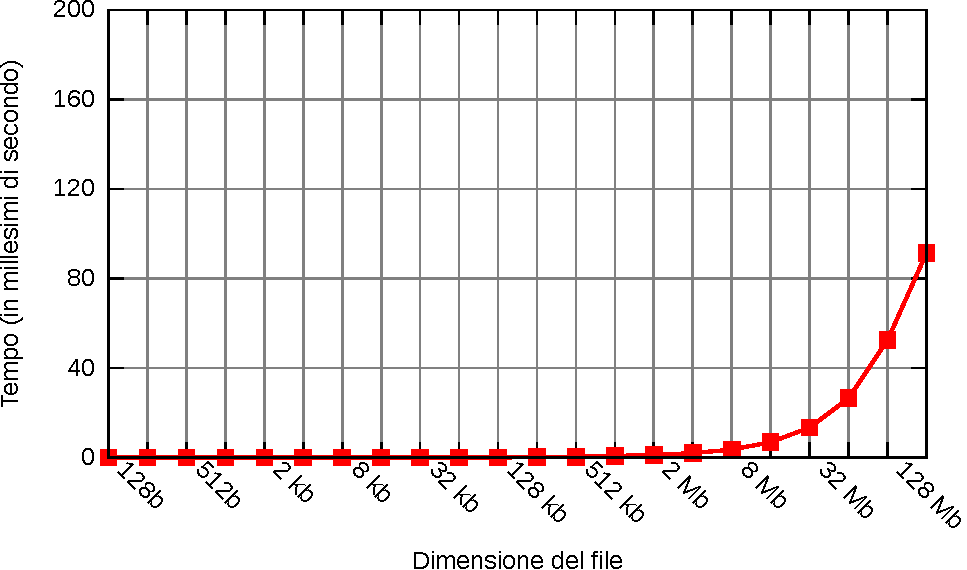
\includegraphics[width=\textwidth]{img/test-read-gpu}
\caption{Tempi di lettura dalla Global Memory della GPU.\label{fig:test-read-gpu}}
\end{center}
\end{figure}

\begin{table}[p]
\begin{center}
\begin{tabular}{|r|r|r|}
\hline
\textbf{Dimensione (byte)} & \textbf{CPU (ms)} & \textbf{GPU (ms)} \\
\hline
128 & 0.003 & 0.018 \\
\hline
256 & 0.004 & 0.020 \\
\hline
512 & 0.004 & 0.021 \\
\hline
1024 & 0.004 & 0.021 \\
\hline
2048 & 0.004 & 0.021 \\
\hline
4096 & 0.007 & 0.022 \\
\hline
8192 & 0.010 & 0.026 \\
\hline
16384 & 0.018 & 0.034 \\
\hline
32768 & 0.032 & 0.046 \\
\hline
65536 & 0.051 & 0.076 \\
\hline
131072 & 0.096 & 0.130 \\
\hline
262144 & 0.182 & 0.246 \\
\hline
524288 & 0.370 & 0.483 \\
\hline
1048576 & 0.759 & 0.952 \\
\hline
2097152 & 1.875 & 1.560 \\
\hline
4194304 & 3.881 & 2.764 \\
\hline
8388608 & 7.219 & 5.121 \\
\hline
16777216 & 13.750 & 9.861 \\
\hline
33554432 & 26.883 & 19.291 \\
\hline
67108864 & 53.088 & 38.644 \\
\hline
134217728 & 107.619 & 76.040 \\
\hline
234700800 & 184.678 & 132.751 \\
\hline
\end{tabular}
\caption{Tempi di scrittura nella Global Memory.\label{tab:test-write}}
\end{center}
\end{table}

\begin{figure}[p]
\begin{center}
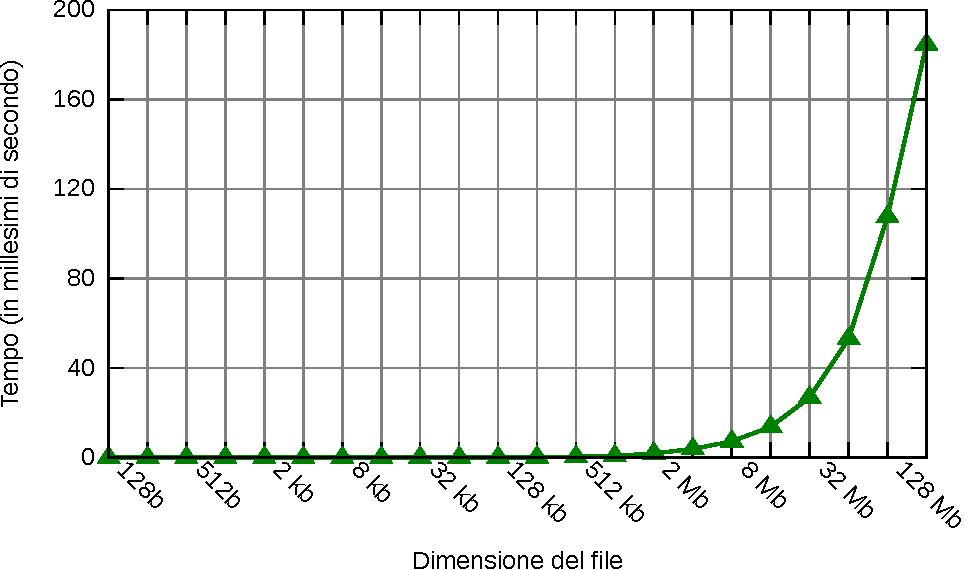
\includegraphics[width=\textwidth]{img/test-write-cpu}
\caption{Tempi di scrittura nella Global Memory della CPU.\label{fig:test-write-cpu}}
\end{center}
\end{figure}

\begin{figure}[p]
\begin{center}
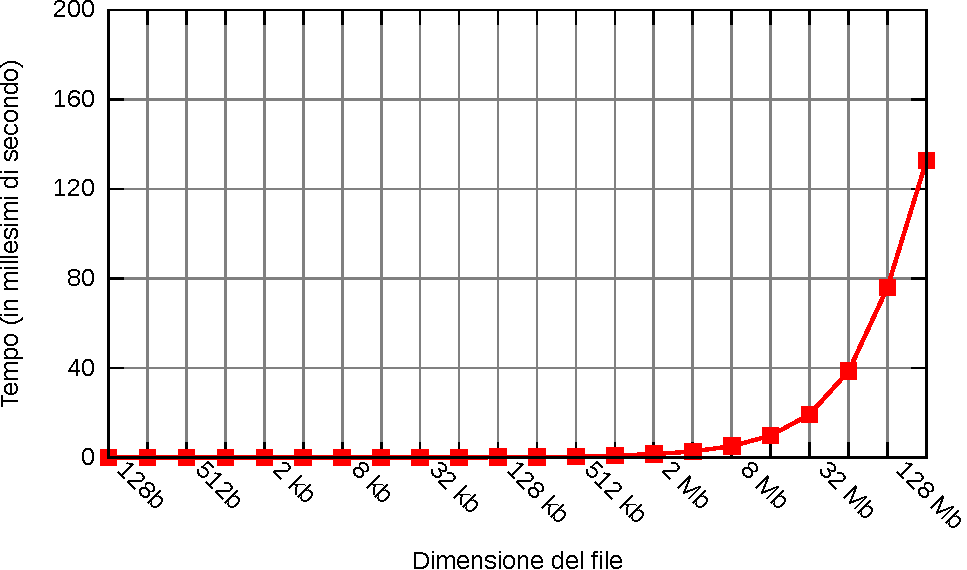
\includegraphics[width=\textwidth]{img/test-write-gpu}
\caption{Tempi di scrittura nella Global Memory della GPU.\label{fig:test-write-gpu}}
\end{center}
\end{figure}

\begin{table}[p]
\begin{center}
\begin{tabular}{|r|r|r|r|}
\hline
\textbf{Dimensione (byte)} & \textbf{CPU (ms)} & \textbf{GPU (ms)} & \textbf{Seriale} \\
\hline
128 & 0.075 & 0.705 & 0.217 \\
\hline
256 & 0.104 & 0.722 & 0.426 \\
\hline
512 & 0.160 & 0.751 & 0.846 \\
\hline
1024 & 0.274 & 0.801 & 1.752 \\
\hline
2048 & 0.286 & 0.905 & 3.415 \\
\hline
4096 & 0.524 & 0.911 & 6.754 \\
\hline
8192 & 0.976 & 0.905 & 13.610 \\
\hline
16384 & 1.883 & 0.948 & 27.128 \\
\hline
32768 & 3.678 & 1.022 & 54.313 \\
\hline
65536 & 7.292 & 1.931 & 113.525 \\
\hline
131072 & 14.492 & 2.936 & 217.586 \\
\hline
262144 & 30.559 & 4.955 & 436.502 \\
\hline
524288 & 57.661 & 8.893 & 869.043 \\
\hline
1048576 & 115.667 & 16.840 & 1741.804 \\
\hline
2097152 & 230.564 & 33.398 & 3484.572 \\
\hline
4194304 & 462.034 & 66.055 & 6995.495 \\
\hline
8388608 & 925.355 & 131.624 & 13995.803 \\
\hline
16777216 & 1850.096 & 262.747 & 27884.374 \\
\hline
33554432 & 3700.182 & 524.854 & 55445.609 \\
\hline
67108864 & 7697.433 & 1049.197 & 111911.418 \\
\hline
134217728 & 15285.159 & 2806.445 & 222053.770 \\
\hline
234700800 & 26178.837 & 6687.997 & 386443.750 \\
\hline
\end{tabular}
\caption{Tempi di cifratura.\label{tab:test-encrypt}}
\end{center}
\end{table}

\begin{figure}[p]
\begin{center}
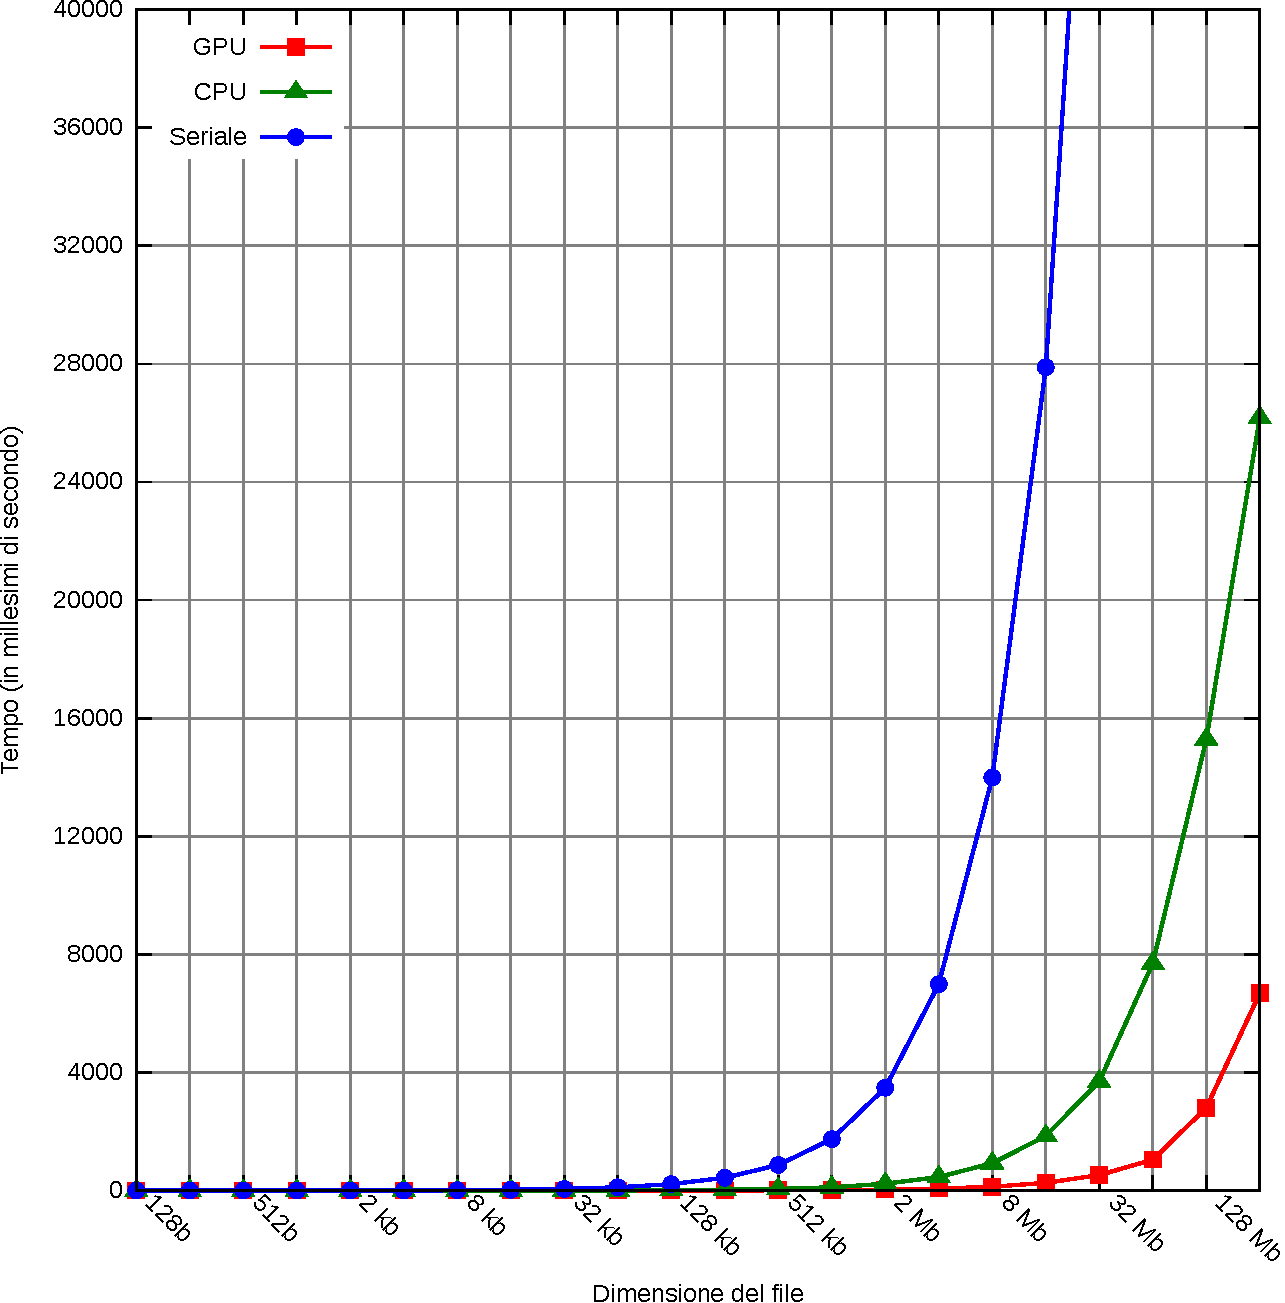
\includegraphics[width=\textwidth]{img/test-encrypt}
\caption{Tempi di cifratura.\label{fig:test-encrypt}}
\end{center}
\end{figure}

\begin{table}[p]
\begin{center}
\begin{tabular}{|r|r|r|r|}
\hline
\textbf{Dimensione (byte)} & \textbf{GPU/CPU} & \textbf{GPU/Seriale} & \textbf{CPU/Seriale} \\
\hline
128 & 0.106 & 0.308 & 2.893 \\
\hline
256 & 0.144 & 0.590 & 4.096 \\
\hline
512 & 0.213 & 1.126 & 5.287 \\
\hline
1024 & 0.342 & 2.187 & 6.394 \\
\hline
2048 & 0.316 & 3.773 & 11.941 \\
\hline
4096 & 0.575 & 7.414 & 12.889 \\
\hline
8192 & 1.078 & 15.039 & 13.945 \\
\hline
16384 & 1.986 & 28.616 & 14.407 \\
\hline
32768 & 3.599 & 53.144 & 14.767 \\
\hline
65536 & 3.776 & 58.791 & 15.568 \\
\hline
131072 & 4.936 & 74.110 & 15.014 \\
\hline
262144 & 6.167 & 88.093 & 14.284 \\
\hline
524288 & 6.484 & 97.722 & 15.072 \\
\hline
1048576 & 6.869 & 103.433 & 15.059 \\
\hline
2097152 & 6.904 & 104.335 & 15.113 \\
\hline
4194304 & 6.995 & 105.904 & 15.141 \\
\hline
8388608 & 7.030 & 106.332 & 15.125 \\
\hline
16777216 & 7.041 & 106.126 & 15.072 \\
\hline
33554432 & 7.050 & 105.640 & 14.985 \\
\hline
67108864 & 7.336 & 106.664 & 14.539 \\
\hline
134217728 & 5.446 & 79.123 & 14.527 \\
\hline
234700800 & 3.914 & 57.782 & 14.762 \\
\hline
\end{tabular}
\caption{Rapporti vari tra i tempi di cifratura.\label{tab:test-ratio}}
\end{center}
\end{table}

\backmatter
\chapter{Conclusioni}

Lo sviluppo di PAES è stata un'ottima occasione per esplorare l'uso delle architetture multi/many-core nell'ambito di un problema reale e, in particolare, l'uso di \ac{OpenCL}. L'esperienza accumulata, oltre ad avallare previsioni ottimistiche sulla crescita di queste tecnologie, può essere in buona parte riutilizzata in progetti futuri, soprattutto nell'ambito dell'esperimento \ac{MaCGO}.

Lo sviluppo di programmi paralleli con \ac{OpenCL} ha una serie di complicazioni: quelle intrinseche nella programmazione parallela e quelle derivanti dalla diversa cura che i vari produttori ripongono nelle loro implementazioni. Per queste ragioni è stato fondamentale sviluppare PAES usando implementazioni \ac{OpenCL} differenti contemporaneamente e corredarlo di una serie di test la cui semplicità d'uso ha reso possibile eseguirli molto spesso.

Nonostante l'uso di \ac{OpenCL} consenta di scrivere programmi in grado di utilizzare in modo trasparente diverse tipologie di dispositivi di calcolo, è stato necessario porre particolare attenzione per sfruttare al meglio le peculiarità degli stessi. Il tipo di adattamento descritto nella sottosezione \ref{subsec:paes-global-local-size} è un modello da seguire anche per altri progetti basati su \ac{OpenCL}. Sempre al fine di rendere un programma \ac{OpenCL} in grado sfruttare al meglio dispositivi eterogenei, è fondamentale strutturarne il parallelismo in modo flessibile e privo di vincoli non strettamente necessari, ove possibile.

Grazie alla natura modulare di PAES, il suo codice potrà essere facilmente integrato e riutilizzato in altri progetti.

\newpage
\addcontentsline{toc}{chapter}{Bibliografia}
\bibliography{bibliografia}{}
\bibliographystyle{unsrt}

\listoftables
\lstlistoflistings
\listoffigures

\end{document}
